\documentclass[13pt]{article}
%\documentclass[a4paper,10pt,twocolumn]{article}
%\documentclass[a4paper,12pt,draft]{article}

\sloppy

\usepackage{cmap}					% поиск в PDF
\usepackage[T2A]{fontenc}			% кодировка
\usepackage[utf8]{inputenc}			% кодировка исходного текста
\usepackage[english,russian]{babel}	% локализация и переносы
\usepackage{amsmath}
\usepackage{amssymb}
\usepackage{amsthm}
\usepackage{graphicx}
\usepackage{float}
\usepackage{subfigure}
\usepackage{color}
\usepackage{url}
\usepackage{ulem}
\usepackage{pdfpages}
\usepackage{biblatex}
\addbibresource{Источник.bib}
\newtheorem{theorem}{Theorem}
\usepackage{tabularx}
\usepackage{nomencl}


\renewcommand{\nomname}{Список используемых сокращений}

\newcommand{\magenta}[1]{\textbf{\textcolor{magenta}{#1}}}
\newcommand{\blue}[1]{\textbf{\textcolor{blue}{#1}}}


\usepackage[a4paper, lmargin={3cm},rmargin={1.5cm},tmargin={2cm},bmargin={2cm}]{geometry}
\usepackage{times}
\usepackage{algorithm}
\usepackage{algpseudocode}
\usepackage{xspace}
\usepackage{lipsum}
\usepackage{pythonhighlight}
\lstnewenvironment{mypython}[1][]{\lstset{style=mypython,#1}}{}

\usepackage{setspace}
\setstretch{1,5}

\setlength{\abovedisplayskip}{0pt}
\setlength{\belowdisplayskip}{0pt}
\setlength{\abovedisplayshortskip}{0pt}
\setlength{\belowdisplayshortskip}{0pt}




\def\l{\delta}
\def\tl{\tilde\delta}
\def\l{\lambda}
\def\tl{\tilde\lambda}
\def\tB{\widetilde B}
\def\tb{\tilde b}
\def\ld{\ldots}

\begin{document}


\includepdf[pages = 1-2]{data/Титульный лист-ВКР-НПМмд_ММИИ.pdf}

\makenomenclature
\newpage



\pagenumbering{arabic}
\newpage

\newpage

\tableofcontents
\nocite{*}   % all not cited bib entrys are shown in bibliography ...


\vspace{-1cm}


\newpage

\includepdf[pages = 1]{data/page.pdf}
\newpage

\section*{Введение}
Эксперименты о временно жизни приобрели популярность в последнее время. Основной целью любого эксперимента о временно жизни является измерение одной или нескольких характеристик надежности рассматриваемых экспериментальных установок. В очень типичной форме эксперимента о временно жизни несколько идентичных элементов испытываются в нормальных условиях эксплуатации и регистрируется «время до отказа» всех элементов. Определение «наработки до отказа» зависит от рассматриваемых элементов. Например, «время до отказа» может быть временем, по истечении которого не достигается минимальная удовлетворительная производительность электронного оборудования, или это может быть количество оборотов, прежде чем шарикоподшипник выйдет из строя. Чтобы проверить срок службы лампочки, «время до отказа» — это количество часов, в течение которых она проработает, прежде чем расплавится. Неисправность может произойти из-за одной или комбинации нескольких из следующих причин: (а) небрежное планирование, (б) некачественное сырье, (в) износ или усталость, вызванные старением изделия и т. д... Поскольку отказ может произойти в любой момент, предполагается, что «время до отказа» является случайной величиной с определенной кумулятивной функцией распределения (CDF).

Так, понятие «обратного момента положительной случайной величины» часто используется для оценки срока службы тех или иных элементов. Обратный момент положительной случайной величины является мерой ее асимметрии. Это может дать представление о распределении времени сбоев или продолжительности жизни продукта или системы. В \cite{mendenhall1960approximation}, отметили, используя метод \textbf{Оценка Максимального Правдоподобия (ОМП)}, что значимость обратного момент при испытаниях о временно жизни зависит от конкретного применения и исходных предположений о распределении времени наработки на отказ. Например, если обратный момент значителен, это говорит о наличии длинного хвоста в левой части распределения, что указывает на большую вероятность ранних отказов или меньшее время жизни. Эта информация может иметь решающее значение для проектирования систем с соответствующим запасом прочности или для оценки надежности изделия в течение ожидаемого срока службы. 

В этой работы, рассмотрили метод аппроксимации значения обратного момента положительной случайной величины. Таким образом, данная работа состоит из трех глав. Первая глава, состоящая из теоретической части. Рассмотрили подробное объяснение статистических моментов и их использования в анализе данных, Формальное определение обратного момента и его роль в характеристике распределения, Сравнение с другими статистическими моментами (средним, дисперсией и т.д.).\\
Второй часть работы будет только в основном рассматривать Интерпретация и смысл использования обратного момент, то есть Анализ последствий обратного момента для понимания данных, Связь между обратным моментом и формой распределения (асимметрия) итак же нескольких конкретные примеры, иллюстрирующие интерпретацию обратного момента в различных контекстах.\\
В третьей главе, будет только в основном, изучить обратный момент в нескольких распределениях, то есть анализ обратного момента в некоторых распределении, влияние обратного момента на асимметричное распределение, а также приведем несколько практических примеров распределений с обратным моментами параллельно.\\
В заключительной главе данного научного исследования подведем итоги, обобщим полученные результаты, практические и теоретические последствия обратного момента, а также наметим дальнейшие перспективы исследований по данной тематике.
 

\newpage
\section*{ОБРАТНЫЕ МОМЕНТЫ СЛУЧАЙНЫХ ВЕЛЕЧИН}\label{section 1}

Некоторые задачи в статистике и других отраслях науки требуют вычисления обратных моментов распределения, также называемых отрицательными или обратными моментами. В статистике примечательными примерами являются задачи о времени жизни и задачи о выборке с выборками случайной длины. Особенно полезны обратные моменты биномиального распределения. Недавние приложения в квантовой физике, например, включают вычисление времени работы некоторых алгоритмов квантовых вычислений, исследование случайных блужданий по n-мерным кубам и точные вычисления доверительной области бета-оценки параметра p биномиального распределения.\par
Целью данной работы является изучение нескольких методов нахождения обратного момента многих статистических распределений, используемых в тестировании жизни и в других научных областях. Многие работы были сделаны, объясняя некоторые практические использования обратного момента. Марко Знидарич дал некоторые иллюстрации использования метода асимптотического расширения для определения обратного момента биномиального и пуассоновского распределений. В. Менденхолл и Э. Х. Леман \cite{mendenhall1960approximation} дают некоторый метод нахождения приближения к обратному моменту, полезный при тестировании жизни, путем нахождения среднего и дисперсии для оценки максимального правдоподобия масштабного параметра распределения Вейбулла, где выборка центрируется в фиксированное время. Позже была проведена более практическая работа в области медицины, где рассматривалась проблема анализа многоцентровых клинических исследований, когда количество пациентов в каждом центре и на каждой линии лечения является случайным и подчиняется распределению Пуассона. В этой работе Валерий Федоров, Байрон Джонс, К. Мэтью Джонс и Анатолий Жиглявский \cite{fedorov2005multi} доказывают реальную важность использования обратного момента распределения Пуассона для определения трех различных оценок разности эффектов лечения, которые обычно используются в многоцентровых клинических исследованиях.


\section{Понимание обратного момента случайных величин}

\subsection{Теоретические основы: случайная величина, ожидаемое значение}\label{theoria}
В статистике перечислены некоторые обычные функции для определения или описания распределения. Случайная величина или случайное число является результатом применения случайных операций. Функция случайной величины или сама переменная по себе является случайной величиной. В противном случае повторение случайной операции $n$ раз приводит к $n$ значениям случайной величины, называемой $\textit{случайная выборка n}$. В соответствии с одним из приведенных выше утверждений, любая функция от этих $n$ чисел сама по себе является случайной величиной.\par
Математическое ожидание ("ожидаемое значение") $E(x)$ по определению является средним значением случайной величины $x$. Стандартное отклонение распределения вероятности оценки $x$ - это стандартная ошибка $x$. Фундаментальным требованием для существования "ожидаемого значения" $E(x)$ является то, что распределение $x$ должно быть произведено случайной операцией. Обратите внимание, что распределение вероятностей представляет собой прогноз относительно размера распределения, которое будет получено для некоторой случайной величины, такой как среднее значение, стандартное отклонение, процентиль или диапазон из 1000 выборок $n$.

\subsection{Определение обратного момента}\label{def}

Предположим, что X на данный момент является положительной случайной величиной. Положим $x \equiv \int_{-\infty}^{0}e^{\frac{t}{x}}dt (x>0),$
\begin{align*}
    E(X) &= \int_{0}^{\infty} xdF(x) = \int_{-\infty}^{0} \int_{0}^{\infty} e^{\frac{t}{x}}dtdF(x)\\
    &= \int_{-\infty}^{0} \int_{0}^{\infty} e^{\frac{t}{x}}dF(x)dt\\
    &= \int_{-\infty}^{0} M_{X-1}(t)dt\\
    &= \int_{0}^{\infty} M_{X-1}(-t)dt\\
    E(X) &= \int_{0}^{\infty} M_{X-1}(-t)dt.\\
\end{align*}

В дальнейшем, величина, обратная $X$, может быть записана как $X ^{-1}$ и рассматриваться как обратный момент случайной величины. По определению, обратный момент случайной величины \(X\) порядка \(r\) определяется как математическое ожидание \(E[X^{-r}]\), где \(r\) - целое число больше нуля. Если случайная величина \(X\) имеет плотность вероятности \(f(x)\), то обратный момент порядка \(r\) вычисляется как:\\
при $X$ - дискретная случайная величина:
\begin{equation*}
    E(X^{-r}) = \sum_{x}x^{-r}P(X).
\end{equation*}
при $X$ является непрерывной случайной величиной:
\begin{equation*}
    E[X^{-r}] = \int_{-\infty}^{\infty} x^{-r} f(x) dx.
\end{equation*}
Обратный момент также можно получить, вычисляя из формулы момента, которая приводит нас к этой формуле, просто заменив $X$ на $X^{-1}$:
\begin{equation}
\label{eq:1}
    E(X) = \int_{0}^{\infty} M_{X}(-t)dt \Longleftrightarrow E(X^{-1}) = \int_{0}^{\infty} M_{X}(-t)dt.
\end{equation}
Так, существует другая формула, специально используемая для дискретной случайной величины. с нетерпением ждем возможности обсудить ее, поскольку наш основной интерес заключается в изучении обратного момента непрерывной случайной величины. Есть два естественных способа обобщить [\ref{eq:1}] на $E(X^{-r})$; один из способов дает\par
\begin{equation}\label{(2)}
    E(X^{-r}) = \int_{0}^{\infty} \int_{t_1}^{\infty} \cdots \int_{t_{r-1}}^{\infty} M_{X}(-t_{r})dt_{r} \cdots dt_2dt_1,
\end{equation}
а другой 
\begin{equation}\label{(3)}
    E(X^{-r}) = \frac{1}{\Gamma(r)^{-1}}\int_{0}^{\infty} t^{n-1}M_{X}(-t)dt.
\end{equation}  
Обратные моменты часто используются в статистике для анализа свойств распределений вероятностей. Они могут предоставить информацию о хвостах распределения и его свойствах. Обратный момент как математическое ожидание имеет свойства, полезные при анализе и решении задач, связанных с вероятностью и статистикой.\\
\underline{Линейность:}
Если \( X \) и \( Y \) - случайные величины, а \( a \) - константа, то обратный момент линейно зависит от случайных величин: 
\[ E\left(\frac{1}{aX} + \frac{1}{y} \right) = \frac{1}{a}E\left(\frac{1}{X}\right) + E\left(\frac{1}{Y}\right). \]
\underline{Сложность:}
Для сложных случайных величин \( Z = g(X, Y) \), где \( g \) - некоторая функция, обратный момент может быть выражен через обратные моменты составляющих случайных величин:
\[ E\left(\frac{1}{Z}\right) = \iint \frac{1}{g(x,y)} f_{X,Y}(x,y) \,dx\,dy. \]
\underline{Условность:}
Для условного обратного момента случайной величины \( X \) при условии \( Y \):
\[ E\left(\frac{1}{X} | Y\right) = \int \frac{1}{x} f_{X|Y}(x|y) \,dx. \]

В этой работе собираемся исследовать задачи нахождения математического ожидания функции и приближения к обратным моментам некоторого распределения. Следует отметить, что обратный момент в анализе данных так же важен, как и положительный, поскольку, принимая во внимание как положительные, так и отрицательные аспекты данных, получаем более сбалансированное и объективное представление о ситуации. Некоторая работа более полно иллюстрирует, что, рассматривая негативные аспекты данных, можно определить области, в которых необходимы улучшения, что может привести к корректирующим действиям для оптимизации производительности. посвящаем в главе [\ref{section 2}], нашей работы дальнейшему описанию его использования в более практических областях. Тем не менее перейдем к изучению обратного момента при дискретных и непрерывных распределениях.
\subsection{Примеры вычисления обратных моментов случайной величины}\label{example}

Прежде чем перейти к методу вычисления обратного момента, очень важно знать, для какого распределения может существовать обратный момент и в соответствии с какими условиями. Вопрос о существовании обратных моментов с непрерывной плотностью вероятности ранее обсуждались Уолтером У. Пьегоршем и Джорджем Казеллой $(1985)$ \cite{piegorsch1985existence}. Позже будем использовать это условие, которое применяется, когда кажется, что распределение непрерывное.\\
Обратный момент также может быть получен из некоторого дискретного распределения случайных величин Ашиш Кумар $(1979)$ \cite{kumar1979negative} разработал интересный пример того, как найти обратный момент для некоторых дискретных распределений, таких как семейство Лагранжевых распределений Пуассона (ЛРП) и Лагранжевых биномиальных распределений (ЛБР).

\subsubsection{Дискретные случайные величины}\label{subSection 1.1}
Трудности, возникающие при вычислении таких выражений, как $E[X^{-1}]$, будут возникать вблизи $X=0$. Пусть X имеет дискретную функцию плотности вероятности с положительной массой при $X = 0$. Было доказано, что $E [X^{-1}]$ будет конечной. Для большего удобства в реальном и понятном примере, пусть $X$ - дискретная случайная величина, имеющая функцию плотности вероятности $f(x)$.\\
A- Если $f(x)$ - вероятность для усеченного биномиального распределения, была полученна Евой Марциняк и Яцеком Веловским \cite{marciniak1999asymptotic} некоторая относительная формула, из которой обозначили при распределении усекаются до нуля:
\begin{equation}
    P(x=k) = \frac{1}{1-q^{n}} \begin{pmatrix}
    n \\
    k
    \end{pmatrix}p^{k}q^{n-k} , \hspace{6 mm} k=\overline{1,n}
\end{equation}
при $q=1-p$, обратный момент может быть задан формулой
\begin{equation}
    f(n) = (1-q^{n})E\Big(\frac{1}{X}\Big)=\sum_{k=1}^{n}\begin{pmatrix}
        n\\
        k
    \end{pmatrix}p^{k}q^{n-k}\frac{1}{k}.
\end{equation}
\underline{Доказательство:}
Пусть $X$ - случайная величина с биномиальным распределением с параметрами n и p. Для вычисления обратного момента будем исходить из определения моментов, поскольку известно, что момент для любого дискретного распределения может быть получен по этой формуле
\[
E(X) = \sum_{x}xP(X=x) \Longleftrightarrow E(X^{-r}) = \sum_{x}x^{-r}P(X=x),
\]
C другой стороны, Чао и Строудерманом (1972) \cite{chao1972negative} и Кресси и др. (1981) \cite{cressie1986moment} был найден другой метод, когда добавляем целое число для получения обратного момента $E(\frac{1}{1+X})$, и этот метод состоит из последовательного интегрирования момент, генерирующий функцию $M_x(t)$ из $X$, обсудим с точки зрения нахождения момента относительно непрерывного распределения.


Чтобы показать, что \[ E[X^{-1}] = \sum_{k=0}^{n} \frac{1}{k} \binom{n}{x} p^x (1-p)^{n-x}, \] из определения \[ E[X^{-r}] = \sum_{k}\frac{1}{k^r} P(X = x) ,\] 

Определим математическое ожидание функции случайной величины:
\[ E[g(X)] = \sum_{k} g(k) P(X = k), \]

Давайте положим, что \( g(k) = k^{-1} \). Тогда у нас есть:
\[ E[X^{-1}] = \sum_{k} \frac{1}{k} P(X = k), \]

Теперь собираемся выразить вероятность \( P(X = k) \) в терминах биномиального распределения:
\[ P(X = x) = \binom{n}{k} p^k (1-p)^{n-k}, \]

Подставив это выражение в формулу для \( E[X^{-r}] \):
\[ E[X^{-r}] = \sum_{k} \frac{1}{k} \binom{n}{k} p^k (1-p)^{n-k}. \]

Вычисление суммы по всем возможным значениям \( k \), суммируем из \( k = 0 \) to \( k = n \), это дает нам возможность $(2)$:
\[ E[X^{-1}] = \sum_{k=0}^{n} \frac{1}{k} \binom{n}{k} p^k (1-p)^{n-k}. \]
B- Если вероятность для пуассоного распределения
\[
P(X=k) = \frac{\lambda^{k}e^{-\lambda}}{k!}, \hspace{6 mm} \textit{при}\ x > 0,  \lambda - \textit{параметр пуассоновкого распределения}.
\]
Тогда обратный момент будет задан следующим образом
\begin{equation}
   E[X^{-1}]  = \sum_{k=1}^{\infty}e^{-\lambda}\frac{\lambda^{k}}{k!}\frac{1}{k},
\end{equation}
\underline{Доказательство:}
Обратный момент данной функции \( E[X^{-1}] = \sum_{k=1}^{\infty}e^{-\lambda}\frac{\lambda^{k}}{k!}\frac{1}{k} \), сначала нам нужно определить обратный момент.

Обратный момент случайной величины \(X\) определяется как \(E[X^{-r}] \), где \( r\) - положительное целое число. В данном случае хотим найти \(E[X^{-1}] \).

Математическое ожидание функции случайной величины \( X\) задается формулой:
\[ E[g(X)] = \sum_{k=1}^{\infty} g(k) P(X=k), \]

Учитывая вероятность \( P(X=k) = \frac{\lambda^{k}e^{-\lambda}}{k!} \), хотим найти \( E[X^{-1}] \), тогда получим:
\[ E[X^{-1}] = \sum_{k=1}^{\infty} \frac{1}{k} e^{-\lambda}\frac{\lambda^{k}}{k!}, \]

Теперь давайте упростим это выражение, переставив термины:
\[ E[X^{-1}] = \sum_{k=1}^{\infty} \frac{1}{k} e^{-\lambda}\frac{\lambda^{k}}{k!} = e^{-\lambda} \sum_{k=1}^{\infty} \frac{\lambda^{k}}{k!k}. \]


Следовательно, Обратный момент данной функции равен \( E[X^{-1}] = e^{-\lambda} \sum_{k=1}^{\infty} \frac{\lambda^{k}}{k!k}. \)

Чтобы обеспечить глубокое понимание обратного момента, в главе 3 этой работы были проведены некоторые практические исследования, которые приведут к получению результатов путем применения различных методов.


\subsubsection{Непрерывные случайные величины }\label{subSection 1.2}
Пусть имеется интеграл Римана вида $\int_{a}^{b}g(x) dx$, где $\big[a, b \big]$ есть конечный интервал, а функция $g(x)$ может становиться бесконечной в конечном числе точек в $\big[a, b \big]$. замечаем, что эти точки называются особыми точками $g(x)$. Если $\int_{a}^{b} g(x) dx$ существует, то это называется сходящимся интегралом, в противном случае он расходится.
\begin{theorem} \label{theorem 1}
    Пусть $g (x)$ и $h (x)$ - неотрицательные функции, являющиеся интегралами Римана от $[c,b]$ для каждого $c$, такие, что $a<c\le b$. Точка $a$ является особенностью для обеих функций.\\ 
Если 
\[
\lim_{x \to a^{+}} \frac{g(x)}{h(x)} = k,
\]
\end{theorem}
где $k$ - положительная константа, а $x \to a^{+}$ обозначает сходимость к $a$ справа, тогда $\int_a^b g(x)dx$ и $\int_a^b h(x)dx$ являются либо сходящимися, либо расходящимися.
Поскольку доказана истинность этой теоремы, можем применить ее только к неотрицательным функциям. Если теорема $1$ верна, и $\int_{a}^{b} h(x)dx$ является либо сходящейся, либо расходящейся, то, то же самое можно сказать и о $\int_a^b g(x)dx$. Случай $k=0$ приводит к одностороннему выводу, что $\int_{a}^{b} g(x)dx$ сходится, если $\int_a^b h(x) dx$ сходится, поскольку здесь существует константа $u$, такая, что $(g(x)/h(x))<1 \textbf{для} a < x < u$, и
\[
\int_a^u g(x)dx<\int_a^uh(x)dx,
\]

если $a$ - единственная особенность для $g(x)$ и $h(x)$, то существование $\int_a^ uh(x)dx$ подразумевает то же самое для $\int_a^ ug(x)dx$. Следовательно, $ \int_a ^ bg (x) dx$ является сходящимся, предполагая, что $g (x)$ интегрируемо по Риману на $ \big [a,b\big]$. Из всего приведенного выше доказательства можем сделать вывод, что из него можно вывести существование первого отрицательного момента.

Пусть X - неотрицательная непрерывная случайная величина с функцией плотности $f(x)$, тогда $E(X ^ {-1})$ существует тогда и только тогда, когда $\int_a^{\delta} (g(x)/x)dx$ сходится для некоторого $\delta > 0.$
Это может быть запись, из которой следует

\[
E\Big(\frac{1}{x}\Big)= \int_0^\infty \frac{f(x)}{x}dx = \int_0^\delta \frac{f(x)}{x}dx + \int_0^\delta \frac{f(x)}{x}dx,
\]
и 
\[
\int_0^\infty \frac{f(x)}{x}dx \le \frac{1}{\delta}\int_\delta^\infty f(x)dx \le \frac{1}{\delta},
\]

где $f(x)$ - непрерывная функция плотности на $(0,\infty)$.
Отметим, что вычисление таких выражений, как $E[\frac{1}{X}]$, будет происходить вблизи $x = 0$. Например, если $X$ имеет дискретную функцию плотности вероятности с положительной массой при $X =0$, $E[\frac{1}{X}]$ будет конечной. Поскольку наша работа относилась к непрерывному случаю, если $f(0) > 0$, то $E[\frac{1}{X}]$ будет бесконечным.\\
\underline{Замечание:}\\
Было проведено много работ, чтобы продемонстрировать условия существования обратных моментов. можем буквально найти некоторые из этих работ, выполненных Уолтером Пьегоршем и Джорджем Казеллой. Для демонстрации существования обратного момента были использованы две фундаментальные теоремы. Рассматривая первое условие обратного момента, которое обозначаем как $ E[X^{-1}],$ должно иметь дискретную или непрерывную вероятность с положительной массой при $X = 0$.\\

Пусть $f(x)$ - непрерывный ФР на $(0, \infty)$, естественно сначала выяснить, является ли $\lim_{x \to 0} f(x) = 0$ достаточным для $E[X^{-1}] < \infty$. Подробно объясним это, применив приведенную ниже теорему.

\begin{theorem} \label{theorem 2}
   Пусть $f(x)$ - непрерывный ФР на $(0, \infty)$. 
Если 
\[
\lim_{x \to 0} \bigg[\frac{f(x)}{x^{\alpha}}\bigg] < \infty, \hspace{6 mm} \alpha > 0, \hspace{6 mm} \text{то} \hspace{6 mm} E[X^{-1}] < \infty.
\] 
\end{theorem}

\underline{Доказательство}:
Если $\alpha > 0$ удовлетворяет теореме \ref{theorem 2}, то существуют конечные константы $M$ и $\delta$, такие, что $|f(x)/x^{\alpha}|\le M$ при $0\le x \le \delta$. Следовательно, 
\[
\int_{0}^{\delta}\frac{f(x)dx}{x} = \int_{0}^{\delta}(x^{\alpha - 1})\frac{f(x)}{x^{\alpha}}dx \\
\le M\int_{0}^{\delta}{x^\{alpha - 1}dx =\frac{M}{\alpha}\delta^{\alpha}.
\]
Следовательно 
\[
E[X^{-1}]<\frac{M}{\alpha}\delta^{\alpha} + \int_{0}^{\delta}\frac{1}{x}{f(x)dx}\\
<\frac{M}{\alpha}\delta^{\alpha} + \frac{1}{\delta}< \infty,
\]
используя непосредственное следствие для дифференцируемых функций плотности из теореме \ref{theorem 2} , можем обозначить следующие.\\ 
\underline{Следствие 2.1.} Пусть $f (x)$ - непрерывный ФР на $(0,\infty)$ с $f(0) =0$. Если $f'(0)$ существует и конечно, то $E[X^{-1}]<\infty.$\\
\underline{Доказательство}: из определения производной,
\begin{equation}
    f'(0) = \lim_{x \to 0}{([f(x) - f(0)]/x)}
    = \lim_{x \to 0}(1/x)f(x),
\end{equation}
поскольку $f(0)= 0$. не можем видеть, что существование $E[X^ {-1}]$ следует из теоремы \ref{theorem 2}, с $\alpha = 1$. Таким образом, некоторым примером может быть проиллюстрировано существование обратного момента.\par
\underline{Пример:}
Гамма-распределение с параметрами $r>0$ и $\lambda>0$ имеет функцию плотности вероятности
\begin{equation}
    f(x) = [\lambda^{r}/\delta(r)]x^{r-1}exp(-\lambda x), \hspace{6 mm} 0\le x\le \infty.
\end{equation}
Где $\delta(.)$ обозначает гамма-функцию. (Экспоненциальное распределение $Exp$, $f(x)=\lambda \textbf{exp}(-\lambda x)$, $0\le x \le \infty$ является частным случаем, поскольку $r=1$.) Легко проверить, что $f(0) > 0 $, если $r\le 1$, что указывает на несуществование $E[X^{-1}]$, если $r \le 1$. Если $r > 1$, то
\[
\lim_{x \to 0}f(x)x^{-(r-1)/2} = 0,
\]
показывающий, что $E[X^{-1}] < \infty$ тогда и только тогда, когда $r>1$.\par
Однако существует пример семейства функций плотности, все из которых нарушают условие существования обратного момента, причем некоторые члены имеют конечный обратный момент, а другие - нет. Уолтер В. Пьегорш и Джордж Казелла (1985) достаточно подробно описывают это с помощью теоремы, которая иллюстрирует, что для $f(x)$ непрерывная плотность на $(0, \infty)$. если $\lim_{x \to 0}(f(x)x^{-\alpha}$ расходиться для всех $\alpha > 0$, то $E[X^{-(1+\delta)}]$ не существует для всех $\delta > 0$.\par
\underline{доказательство:}
Используя интегрирование по частям, обозначаем
\[
\int_{0}^{t}\frac{f(x)}{x^{(1+\delta)}}dx = \lim_{\epsilon \to 0}\int_{\epsilon}{t}\frac{f(x)}{x^{1+\delta}}dx \\
= \lim_{\epsilon \to 0}\Bigg\{\bigg[\frac{F(x)}{x^{1+\delta}}\bigg]_{\epsilon}^{t} + \int_{\epsilon}{t}\frac{(1+\delta)F(x)}{x^{2+\delta}}dx\Bigg\},
\]
поскольку $F(x)$ не уменьшается, имеем $F(x)\ge F(\epsilon)$ on $(\epsilon,t);$ следовательно
\[
    \lim_{\epsilon \to 0}\int_{\epsilon}{t}\frac{f(x)}{x^{1+\delta}}dx \ge \lim_{\epsilon \to 0}\Bigg\{\bigg[\frac{F(x)}{x^{1+\delta}}\bigg]_{\epsilon}^{t} + (1 + \delta)F(\epsilon)\int_{\epsilon}^{t}\frac{dx}{x^{2+\delta}}\bigg]\Bigg\}
\]
\[
 = \lim_{\epsilon \to 0}\Bigg\{ \frac{F(t)}{t^{1+\delta}} - \frac{F(\epsilon)}{t^{1+\delta}}\Bigg\} = \frac{F(t)}{t^{1+\delta}},
\]
таким образом, имеем
\[
\int_{0}^{t}\frac{f(x)}{x^{1+\delta}}dx > \frac{F(t)}{x^{1+\delta}}.
\]
используя гипотезу теоремы вместе с правилом Лопиталя, имеем $F(t)/t^(1+\delta) \to {\infty} \textbf{as} t \to 0,$ показывающий несуществование $E[X^{-(1+\delta)}]$. пришли к выводу, что для непрерывной, позитивной функции $f$, ограниченное значение, близкое к нулю, означает, что $E[X^{-\alpha}]$ существуют для каждого $0 < \alpha < 1$;
\[
\lim_{x \to 0}f(x)/x^{\alpha} < \infty.
\]
Для некоторых $\alpha > 0$ подразумевает, что $E[X^{-1}]<\infty$; и $\lim_{x \to 0}f(x)/x^{\alpha} = \infty $ для каждого $\alpha > 0$ подразумевает, что $E[X^{-(1 + \delta)}] =  \infty$ для каждого $\delta > 0$. 
\newpage
\section*{ОБРАТНЫЕ МОМЕНТЫ НЕКОТОРЫЕ РАСПРЕДЕЛЕНИЯ}
\section{Численное решение обратных моментов некоторых распределениях}\label{section 2}
\subsection{Обратные моменты некоторых дискретных распределений}
Как уже упоминалось в главе [\ref{section 1}] нашей работы, обратные моменты играют большую роль в повседневной жизни, в частности, в нескольких стратегиях, поскольку они влияют на оценку рисков, страхование и финансы, и это важная концепция вероятности. Изучение обратных моментов основано на случайных выборках, $X$ - это количество наблюдений $Z_{1}, Z_{2}, \cdots, Z_{x}$, где обратные моменты были идентифицированы как $E(\frac{1}{x^{r}})$ из определения [\ref{eq:1}].\par
В этом главе и для упрощения методы получения обратных моментов распределений, на которых будем основывать наше исследование, воспользуемся методом Чао и Строудермана (1972)\cite{chao1972negative}, согласно которому определяется обратный момент $E\bigg[\frac{1}{(A + x)^{r}}\bigg]$, где $X + A > 0$ и также $r$ является неотрицательным целым числом.

\subsubsection{Обобщенная геометрическая случайная величина с обратным моментом}\label{subsection 2.1}

Предположим, что $X$ - обобщенная геометрическая случайная величина с параметрами $\lambda$, имеющими функцию вероятностной массы
\begin{equation}
    P_{x}(\lambda) = x\lambda^{x-1}(1-\lambda)^{2}, \hspace{6 mm} x= 1,2,\cdots,\\
\end{equation}
\textit{где} $0<\lambda<1$. 
Было доказано, что определение обобщенного гипергеометрического ряда дается по следующей формуле:
\[ {}_pF_q(a_1, \ldots, a_p; b_1, \ldots, b_q; z) = \sum_{n=0}^{\infty} \frac{(a_1)_n \cdots (a_p)_n}{(b_1)_n \cdots (b_q)_n} \frac{z^n}{n!}, \]

где \( (a)_n \) обозначает символ Почхаммера или возрастающий факториал, определяемый как \( (a)_n = a(a+1)\ldots(a+n-1) \) с \( (a)_0 = 1 \). Параметры \( a_i \) и \( b_i \) являются комплексными числами, а \( z\) - комплексной переменной. Ряд сходится для определенных значений \( z\) и соответствующих параметров. Давайте сначала докажем, как получить эту формулу:
\[ 
{}_pF_q(a_1, \ldots, a_p; b_1, \ldots, b_q; z) =  \sum_{n=0}^{\infty} \frac{(a_1)_n^{r} \cdots (a_p)_n^{r}}{(b_1)_n^{r} \cdots (b_q)_n^{r}} \frac{z^n}{n!}
\]
\[
= 1 + \frac{a_{1}^{r}*a_{2}^{r} \cdots a_{p}^{r}}{b_{1}^{r}*b_{2}^{r} \cdots b_{p}^{r}}z + \frac{[a_{1}(a_{1}+1)]^{r}[a_{2}(a_{2}+1)]^{r} \cdots [a_p(a_p + 1)]^{r}z^2}{b_{2}(b_{2}+1)]^{r} \cdots [b_p(b_p + 1)]^{r}2!} + \cdots
\]
где $(\lambda_i)_n^r = (\lambda_i)^r(\lambda_i+1)^r(\lambda_i+2)^r \cdots (\lambda_i + n - 1)^r$, $(\lambda_i)_0^r = 1$, $i = 1,2,\cdots,p.$\\
Если  $r=1$ тогда $${}_pF_q(a_1, \ldots, a_p; b_1, \ldots, b_q; z) = \sum_{n=0}^{\infty} \frac{(a_1)_n \cdots (a_p)_n}{(b_1)_n \cdots (b_q)_n} \frac{z^n}{n!},$$ является гипергеометрическим рядом. Обратный момент обобщенной геометрической случайной величины можно получить, применив приведенную ниже теорему (2.1).\\

\begin{theorem}
    Предположим, что $X$ является обобщенной геометрической случайной величиной с параметрами $\lambda$ для $0<\lambda<1$, тогда обратный момент $r\textit{-ого}$ порядка задается формулой
\[
E\bigg(\frac{1}{(X+A)^r}\bigg)= \frac{(1-\lambda)^2}{(A+1)^r}{}_2F_{1}[(A+1,r),2;(A+2,r);\lambda],
\]
где $\textbf{А}\ge 0$.
\end{theorem} 
\underline{Доказательство:} Согласно определению 1, тогда
\begin{align*}
    E\bigg(\frac{1}{(X+A)^r}\bigg) &= \sum_{x=1}^{\infty}x\lambda^{x-1}(1-\lambda)^{2}\frac{1}{(x+A)^r}\\
    &= \frac{(1-\lambda)^2}{(A+1)^r}+\frac{2\lambda(1-\lambda)^2}{(A+2)^r}+\frac{3\lambda^2(1-\lambda)^2}{(A+3)^k}+ \cdots \\
    &= \frac{(1-\lambda)^2}{(A+1)^r}\Bigg\{1+\frac{2(A+1)^r}{(A+2)^r}\frac{\lambda}{1!}+\frac{2*3(A+1)^r(A+2)^r}{(A+2)^r(A+3)^r}\frac{\lambda^2}{2!}+\cdots\Bigg\} \\
    &= \frac{(1-\lambda)^2}{(A+1)^r}\sum_{n}^{\infty}\frac{(A+1)_{n}^{r}(2_n)}{(A+2)_{n}^{r}}\frac{\lambda^{n}}{n!},
\end{align*}
\begin{equation}\label{eq:9}
    E\bigg(\frac{1}{(X+A)^r}\bigg) = \frac{(1-\lambda)^2}{(A+1)^r}{}_2F_1 \Big[(A+1,r),2;(A+2,r);\lambda \Big].
\end{equation}
следует отметить, что при $r=1$ также получаем первый обратный момент для обобщенной геометрической случайной величины с параметрами $\lambda$ для $0<\lambda<1$ и можем вычислить его по формуле:
\[
E\bigg(\frac{1}{X+A}\bigg)=\frac{(1-\lambda)^2}{A+1}{}_2F_{1}\Big[A+1,2;A+2;\lambda\Big]
\]
\underline{Пример:}
Для любой случайной величины X - обобщенной гипергеометрической, распределенной с параметрами $\lambda = 3$, найдите первый и второй обратные моменты, когда $X+A>0$. Можно предположить, что эти  целые числа $a,b, c,z = 1,2,\cdots,$.

1- Чтобы, найти первый обратный момент обобщенного гипергеометрического распределения случайной величины \(X\), зададим параметры \(A = 1\) и \( \lambda = 3\), используя приведенную формулу, подставим заданные значения в формулу. Формула такова:

\[ E\left(\frac{1}{X+A}\right) = \frac{(1-\lambda)^2}{A+1} {}_2F_{1}\left[A+1,2;A+2;\lambda\right]. \]

Учитывая, что \( A = 1 \) and \( \lambda = 3 \), формула становится:

\[ E\left(\frac{1}{X+1}\right) = \frac{(1-3)^2}{1+1} {}_2F_{1}\left[1+1,2;1+2;3\right] = \frac{(-2)^2}{2} {}_2F_{1}\left[2,2;3;3\right]. \]

Теперь еще больше упростим это выражение. Обобщенная гипергеометрическая функция \( {}_2F_{1} \) может быть рассчитан следующим образом:

\[ {}_2F_{1}(a,b;c;z) = \sum_{r=0}^{\infty} \frac{(a)_r (b)_r}{(c)_r} \frac{z^r}{r!}, \]

Где \( (x)_r \) обозначает символ Почхаммера, определяемый как \( (x)_r = x(x+1)(x+2)...(x+r-1) \).

В нашем случае у нас есть:

\[ {}_2F_{1}(2,2;3;3) = \sum_{r=0}^{\infty} \frac{(2)_r (2)_r}{(3)_r} \frac{3^r}{r!}. \]

Теперь подставим эти значения в формулу и вычислим первый обратный момент обобщенного гипергеометрического распределения для заданных параметров.\par

\[ E\left(\frac{1}{(X+1)^r}\right) = \frac{(-2)^2}{2} {}_2F_{1}\left[2,2;3;3\right] \]
\[
\Longleftrightarrow  E\left(\frac{1}{(X+1)^r}\right) = \frac{(-2)^2}{2} {}_2F_{1}\sum_{r=0}^{\infty} \frac{(2)_r (2)_n}{(3)_r} \frac{3^r}{r!}.
\]

2- Чтобы, найти второй обратный момент \(r= 2\) обобщенного гипергеометрического распределения случайной величины, где \(A = 1\) и \(\lambda = 3\), используя приведенную вами формулу, нам нужно подставить заданные значения в формулу.

\[ E\left(\frac{1}{(X+A)^r}\right) = \frac{(1-\lambda)^2}{(A+1)^r}{}_2F_1 \left[(A+1,r),2;(A+2,r);\lambda \right] \]

подставим заданные значения в формулу:

\[ E\left(\frac{1}{(X+1)^2}\right) = \frac{(1-3)^2}{(1+1)^2}{}_2F_1 \left[(1+1,2),2;(1+2,2);3 \right] \]

давайте упростим выражение:

\[ E\left(\frac{1}{(X+1)^2}\right) = \frac{(-2)^2}{2^2}{}_2F_1 \left[ (2,2), 2; (3,2); 3 \right] \]

\[ E\left(\frac{1}{(X+1)^2}\right) = \frac{4}{4}{}_2F_1 \left[ 2, 2; 3; 3 \right] \]

Теперь рассчитаем обобщенную гипергеометрическую функцию \({}_2F_{1}\) для заданных параметров \((a,b;c;z)\) и получим 
\[ 
E\left(\frac{1}{(X+1)^2}\right) =  \sum_{r=0}^{\infty} \frac{(2)_r (2)_r}{(3)_r} \frac{3^r}{r!} = \sum_{r=0}^{\infty} \frac{(2)_2 (2)_2}{(3)_2} \frac{3^2}{2!}
\]

Подставляя \(r=2\) в формулу, получаем:

\[ \frac{(2)_2 (2)_2}{(3)_2} \frac{3^2}{2!} \]

Теперь давайте вычислим значения:

1. \((2)_2 = 2 \times 1 = 2\) 
2. \((3)_2 = 3 \times 2 = 6\)
3. \(2! = 2 \times 1 = 2\)


Решение этого выражения дает нам:

\[ \frac{4}{6} \times 9 = \frac{2}{3} \times 9 = 6 \]

Следовательно, \(E\left(\frac{1}{(X+1)^2}\right)\) для \(r=2\) равно 6.
\subsubsection{Биномиальное распределение случайной величины с обратным моментом}\label{subsection 2.2}
В этом разделе собираемся изучить обратные моменты положительного биномиального распределения. Предположим, что X - положительная случайная величина, биномиально распределена с параметрами $n$ и $p$, то есть можно записать что 
\begin{equation}\label{eq:(10)}
    P\big(X=k\big) = \binom{n}{k} p^{k} q^{n-k}, \hspace{6 mm} k=0,\cdots,n
\end{equation}
или также можно писать в виде суммы для вычислительной функции
\begin{equation*}\label{eq:(11)}
    P\big(X \le i\big) = \sum_{k=0}^{n} \binom{n}{k} p^{k} q^{n-k}, \hspace{6 mm} i=1,\cdots, n
\end{equation*}
где $q=1-p$, $r-$ого порядка обратного момента задается формулой
\begin{equation}\label{eq:(12)}
   E\bigg(\frac{1}{X^{r}}\bigg) =  \sum_{k=i}^{n} \binom{n}{k} p^{n}q^{n-k} \frac{1}{k^r}.
\end{equation}

Как упоминали в разделе [\ref{example}], однако легко найти первой обратный момент ну сложности начинается когда следует найти гораздо больше степени обратного момента биномиального распределения. Тем не мене воспользуемся его, чтобы найти первой обратный момент биномиального распределения. Чтобы всем было легче, перепишем нашу формулу, используя метод М. Т. Чао и У. Э. СТРОУДЕРМАНА, таким образом, получим эту новую формулу.
\[
 E\bigg(\frac{1}{(X+A)^{r}}\bigg) =  \sum_{k=i}^{n} \binom{n}{k} P^{n}q^{n-k} \frac{1}{(k+A)^r},
\]
где $X+A>0$. Предположим, что $A=1$, а для первого обратного момента также предположим, что $r=1$, тогда имеем
\[
 E\bigg(\frac{1}{X+1}\bigg) =  \sum_{k=i}^{n} \binom{n}{k} P^{n}q^{n-k} \frac{1}{k+1},
\]
используя биномиальную теорему, простая алгебра показывает, что:
\[
\frac{1}{k+1}\binom{n}{k}=\frac{1}{n+1}\binom{n+1}{k+1},
\]
заменив это в формуле, получим
\[
 E\bigg(\frac{1}{X+1}\bigg)= \frac{1}{n+1}\sum_{0}^{n}\binom{n+1}{k+1}p^{k}(1-p)^{n-k},
\]
пусть умножается на $\frac{1}{p}$:
\[
E\bigg(\frac{1}{X+1}\bigg)= \frac{1}{p(n+1)}\sum_{k=0}^{n}\binom{n+1}{k+1}p^{k+1}(1-p)^{n+1-(k+1)},
\]
установим $k+1=i$ и получим,
\begin{align}
E\bigg(\frac{1}{X+1}\bigg)   &=\frac{1}{p(n+1)}\sum_{i=1}^{n+1}\binom{n+1}{i}p^{i}(1-p)^{n+1-i}, \\
&=\frac{1}{p(n+1)}\Bigg(-(1-p)^{n+1}+\sum_{i=o}^{n+1}\binom{n+1}{j}p^{i}(1-p)^{n+1-i}\Bigg),
\end{align}
из биномиальной теоремы можем обозначить, что
\[
\sum_{i=0}^{n+1}Pr(Bin(n+1,p)=i)=\sum_{i=0}^{n+1}\binom{n+1}{i}p^{i}(1-p)^{n+1-i}=1.
\]
\underline{Доказательство:}

Теперь, используя биномиальную теорему, знаем, что:

\[ (x+y)^{n} = \sum_{i=0}^{n} \binom{n}{i} x^{i} y^{n-i}, \]

Если позволим \( x = p \) и \( y = 1-p \), можем переписать приведенную выше сумму следующим образом:

\[ (p + (1-p))^{n+1} = 1^{n+1} = 1, \]

Следовательно,

\[ \sum_{i=0}^{n+1} Pr(Bin(n+1,p)=i) = \sum_{i=0}^{n+1} \binom{n+1}{i} p^i (1-p)^{n+1-i} = 1, \]
давайте заменим его в (13), и получим
\begin{equation}\label{14}
    E\bigg(\frac{1}{X+1}\bigg)=\frac{(1-(1-p)^{n+1})}{p(n+1)}=\frac{1-q^{n+1}}{p(n+1)}.
\end{equation}
Первый обратный момент может быть получен буквально из формулы [\ref{14}]. Однако этот метод не является простым для вычисления высших степеней обратного момента для биномиального распределения. Поэтому собираемся использовать другой подход для продолжения наших исследований.\par
 Для простоты, как и прежде, будем выводить значения в терминах степеней, обратных $(np + q)$. предполагаем, что $r$ - произвольное действительное и положительное целое число, заметим, что именно при достаточно резком распределении обратный момент будет приблизительно задаваться величиной, обратной среднему значению, $E(1/X^{r})\approx 1/E(X)^r$. Если распределение не равно нулю в одной точке, то этот результат является точным. Обзор проблемы обратных моментов, $ (1945)$ Стефан \cite{stephan1945expected} изучал первый и второй моменты для биномиального распределения. $(1963)$ Заккула Говиндараджулу \cite{govindarajulu1963recurrence} также нашел рекурсивную формулу для обратных моментов биномиального распределения. Однако рекурсивная формула довольно сложна, поскольку она включает рекурсию в $n$, а также в силу момента $r$. И, как видим, формулу [\ref{eq:(11)}] в терминах, нелегко вычислить при больших значениях $np$. Нужно суммировать множество слагаемых, каждое из которых является произведением очень малого и очень большого числа, и все это вместе приводит к небольшому обратному моменту. $ (1972)$ Чао и Строудерман рассмотрели несколько иные обратные моменты, определяемые как $E(1/(X+ A)^r)$, которые часто легче вычислить. Получены простые выражения для целых чисел $A \ge 1$ и $r = 1$. К общей формуле были выведены некоторые общие ряды и два способа обобщения $E(1/(x+ A)^r)$.
\begin{equation}\label{12}
    E\Big(\frac{1}{(X+A)^{r}}\Big) = \frac{1}{\Gamma(r)}\int_{0}^{\infty}t^{r-1}e^{-At}M(-t)dt .
\end{equation}
где $M(t)$ это производящая функция моментов, $M(t)=E(e^{tx})=\sum_{k=0}^{\infty}\frac{\mu_{r}x^{r}}{r!}$ с $\mu_r = E(x^{r})$.
Однако, прежде чем продолжить, давайте докажем две вспомогательные леммы о центральных моментах.\par
\underline{Лемма 1 :}\label{theorem}
Пусть $M(t)$ - производящая функция распределения вероятностей,
\begin{equation}
    M(t) = \sum_{k=0}^{\infty}\mathbf{E}(x^{k})\frac{t^{k}}{k!},
\end{equation}
где $\mathbf {E}(x^{k})$ - это $k$-ого момент относительно начала координат. Тогда производящая функция $F(t)$ центральных моментов,
\[
F(t)= \sum_{k=0}^{\infty}\mu_{k}\frac{t^{k}}{k!}, \hspace{6 mm} \mu_{k}:=\mathbf{E}((x-\mathbf{E}(x))^k),
\]
где $\mathbf{E}(x)$ - среднее значение. задается формулой
\[
F(t) = e^{-t\mathbf{E}(x)}M(t).
\]\
\underline{Доказательство:} Лемма доказывается простым разложением,
\[
F(t) = \sum_{k = 0}^{\infty}\sum_{l=0}^{\infty}(-\mathbf{E}(x))^{l}\frac{t^{l}}{l!}\mathbf{E}(x^{k})\frac{t^{k}}{k!}.
\]
Переписывание суммирования в терминах $j=l +k$ и $l$ и распознавание биномиального разложения $(x-\mathbf{E}(x))^{j}$, получаем $F(t)=\sum_{j=0}^{\infty}\mu_{j}t^{j}/j!$.
Применив [\ref{theorem}] биномиальное распределение, получаем:\par
\underline{Следствие 1:} Для биномиального распределения производящая функция $F_{n}(t)$ центральных моментов равна,
\[
F_{n}(t)=(qe^{-tp} + pe^{tq})^n,
\]
где центральными моментами являются
\[
\mu_{k}(n)=\sum_{i=0}^{n}\binom{n}{i}p^{i}(1-p)^{n-i}(i-np)^{k}.
\]

\underline{Доказательство:} Производящая функция моментов положительного биномиального распределения $M_{n}(t)=(pe^{t}+ q)^{n}$. Используя лемму 1 в нашем подходе, поскольку $X$ распределен биномиально, генерирующий момент будет доказано по этой формуле
\begin{align*}
M(t) &= E(e^{tk}) = \sum_{k=0}^{\infty}\frac{\mu_{k}x^{k}}{k!}, \\
     &= \sum_{k=0}^{n}\binom{n}{k}p^{k}(1-p)^{n-k}e^{tk},\\
 M(t)    &=\sum_{k=0}^{n}\binom{n}{k}(pe^{t})^{k}(1-p)^{n-k},
\end{align*}
применяя биномиальную теорему, получаем
\[
 M(t) = (pe^{t}+(1-p))^{n} = (pe^{t}+ q)^{n}.
\]   
Итак воспользуемся формулой [\ref{eq:1}] для того чтобы  найти первый обратный момент 
\begin{equation*}
     E(X^{-1}) = \int_{0}^{\infty} M_{X}(-t)dt \Longleftrightarrow E(X^{-1}) = \int_{0}^{\infty} (pe^{-t}+ q)^{n}dt.
\end{equation*}
Интеграл можно решать через биномиальную теоремую  Таким образом, интеграл становится:
\begin{align*}
    E\bigg(\frac{1}{X}\bigg) &= \int_{0}^{\infty}\bigg[ \binom{n}{0}\big(pe^{-t} \big)^{n} + \binom{n}{1} \big(pe^{-t} \big)^{n-1}q + \cdots + \binom{n}{n-1}\big(pe^{-t} \big)q^{n-1} + \binom{n}{n}q^{n} \bigg]dt,\\
    &= \binom{n}{0} \int_{0}^{\infty}\big(pe^{-t} \big)^{n} dt + \binom{n}{1} \int_{0}^{\infty} \big(pe^{-t} \big)^{n-1}q dt  + \cdots + \binom{n}{n-1} \int_{0}^{\infty} pe^{-t} q^{n-1} dt + q^{n} \int_{0}^{\infty} dt.
\end{align*} 
Проанализируем решение интеграла шаг за шагом. Обратившись к последнему члену интеграла:
\[
 q^{n} \int_{0}^{\infty} dt = q^{n} t \Bigg]_{0}^{\infty}.
\]
Последное слагаемое интеграла явно расходится при $t \to \infty$. Таким образом, мы можем предположить, что интеграл не имеет конечного значения; он либо стремится к бесконечности, либо сходится к нулю в зависимости от членов разложения. 
Следовательно, он не может быть непосредственно вычислен как определенный интеграл.
Таким обрзаом при $t \to \infty$, также  $E(X^{-1}) \to -\infty$. Поэтому трудно найти первой обратный момент положительного биномиального распределения. 

Многие работы были сделаны, для того чтобы найти обратный момент положительного биномиального распределения когда представляем что обратной момент принимаем  $E(X^{-1}) \approx E(\frac{1}{X+A})$. рассматриваем такие примеры в работе  \cite{chao1972negative}, когда имеем что  $X$ биномиальная случайная величина, при такой что производящая функция распределения можно $X+A-1$, где $X+A>\delta>0$. также будем исследовать  этот метод, для того чтобы выразить первый обратный момент.
Давайте используем эту формулу в [\ref{12}] и одновременно заменим $\Gamma(r)= (r-1)!$ на ее значение, и тогда получим:
\begin{equation*}
    E\Big(\frac{1}{(X+A)^{r}}\Big) = \frac{1}{\Gamma(r)}\int_{0}^{\infty}t^{r-1}e^{-At}M(-t)dt 
    \Longleftrightarrow
     E\Big(\frac{1}{(X+A)^{r}}\Big) = \frac{1}{(r-1)!}\int_{0}^{\infty}t^{r-1}e^{-At}(pe^{t}+ q)^{n}dt
\end{equation*}
при $r=1$, получим у нас формула первой обратный момент положительного биномиального распределения 
\begin{equation*}
   E\Big[\frac{1}{X+A}\Big] = \int_{0}^{\infty} e^{-At}M(-t)dt \Longleftrightarrow E\Big(\frac{1}{(X+A)}\Big) =  \int_{0}^{\infty}e^{-At}(pe^{t}+ q)^{n} dt.
\end{equation*}
И так интеграл можно записать 
\begin{align*}
  E\Big[\frac{1}{X+A}\Big] &=  \int_{0}^{\infty} \Bigg[\binom{n}{0}\Big(\big(pe^{-t}\big)^{n}\Big)e^{-At}  +\cdots 
    +\binom{n}{n-1}\big(pe^{-t}\big)q^{n-1} e^{-At} 
    +\binom{n}{n}q^{n} e^{-At}\Bigg]dt ,\\ 
    &=\binom{n}{0}p^{n} \int_{0}^{\infty}e^{-nt} e^{-At}dt + \cdots+ \binom{n}{n-1}pq^{n-1} \int_{0}^{\infty}e^{-t} e^{-At} dt + \binom{n}{n}q^{n} \int_{0}^{\infty} e^{-At}dt ,\\
    &=\binom{n}{0}p^{n} \int_{0}^{\infty}e^{-t(n+A)}dt + \cdots+ \binom{n}{n-1}pq^{n-1} \int_{0}^{\infty}e^{-t(A+1)} dt + \binom{n}{n}q^{n} \int_{0}^{\infty} e^{-At}dt ,\\
   &=-\Bigg[\binom{n}{0}p^{n}\Big[\frac{1}{n+A}e^{-t(n+A)}\Big]_{0}^{\infty}  + \cdots+\binom{n}{n-1}pq^{n-1}\Big[\frac{1}{A+1}e^{-t}\Big]_{0}^{\infty}+ q^{n}\Big[\frac{e^{-At}}{A}\Big]_{0}^{\infty} \Bigg] ,\\
 E\Big[\frac{1}{X+A}\Big]  &=  \frac{p^{n}}{n+A} + \binom{n}{1}\frac{P^{n-1}q}{n+A+1}+ \cdots +  \binom{n}{n-1}\frac{pq^{n-1}}{A+1}+ \frac{q^{n}}{A}.
\end{align*}

Отметим что, при $A=1$, получим первой обратный момент биномиального распределения так и в [\ref{14}]:
\[
 E\Big[\frac{1}{X+1}\Big]  =  \frac{p^{n}}{n+1} + \binom{n}{1}\frac{P^{n-1}q}{n+2}+ \cdots +  \binom{n}{n-1}\frac{pq^{n-1}}{2} + q^{n},
\]
\[
 E\bigg(\frac{1}{X+1}\bigg)=\frac{(1-(1-p)^{n+1})}{p(n+1)}=\frac{1-q^{n+1}}{p(n+1)}.
\]
При $A=2$ так же получим что,
\[
 E\Big[\frac{1}{X+2}\Big]  =  \frac{p^{n}}{n+3} + \binom{n}{1}\frac{P^{n-1}q}{n+2}+ \cdots +  \binom{n}{n-1}\frac{pq^{n-1}}{3} + \frac{q^{n}}{2}
\]
\[
 E\Big[\frac{1}{X+2}\Big] = \frac{1}{(n+1)p}\Big[1- \frac{(1-q^{n+2})}{(n+2)p} \Big].
\]
 так же выполнения изменений переменных выводит альтернативное рекурсивное выражение найдено в работе Чао и Строудермана (1972), можем вывести что:  
\begin{align*}
   E\Big(\frac{1}{(X+A)^{r}}\Big) &= \frac{1}{(r-1)!}\int_{0}^{\infty}t^{r-1}e^{-At}(pe^{t}+ q)^{n}dt, \\
    &=\int_{0}^{\infty}\frac{t^{r-1}}{(r-1)!}e^{-At}(pe^{t}+ q)^{n}dt .\\
\end{align*}

Прежде чем продолжить наше исследование, давайте сначала приведем несколько примеров преобразований Лапласа и их обратных формул

\vspace{6 mm}
\begin{center}
\begin{tabular}{|c|c|}
\hline
     $L_w(x)$ & $w(z)$ \\
\hline
$x^{-n}$ & $z^{n-1}/(n-1)!$, $\hspace{3 mm}$ $n=1,2,\cdots$ \\
$x^{-1/2}$ & $(\pi z)^{-1/2}$ \\
$x^{-3/2}$ & $2(z/\pi)^{1/2}$ \\
$x^{-(n+1/2)}$ & $\frac{2^n z^{n-1/2}}{1*3\cdots(2n-1)\pi^{1/2}}$, $\hspace{3 mm}$ $n=1,2,\cdots$ \\
$\Gamma(\mu)/x^{\mu}$ & $z^{\mu-1},$ $\hspace{3 mm} \mu>0$ \\
$\Gamma(\mu)/(x+a)^{\mu}$ & $z^{\mu-1}e^{-az},$ $\hspace{3 mm} \mu>0$\\
$(x^2 - a^2)^{-1}$ & $a^{-1}sinh(az)$ \\
$log(1+a/x)$ & $z^{-1}-z^{-1}e^{-az}$\\
\hline
\end{tabular} 
\end{center}


\vspace{6 mm}
Можно тогда переписать заменяя через таблицу Лапласа, и получим тогда 
\begin{align*}
   E\Big(\frac{1}{(X+A)^{r}}\Big) &=\int_{0}^{\infty}\frac{t^{r-1}}{(r-1)!}e^{-At}(pe^{t}+ q)^{n}dt \Longleftrightarrow E\Big(\frac{1}{(X+A)^{r}}\Big) = \int_{0}^{\infty} \frac{\Gamma(r)}{(r-1)!(t+A)^{r}}(pe^{t}+ q)^{n}dt, \\
   E\Big(\frac{1}{(X+A)^{r}}\Big) &= \int_{0}^{\infty}\frac{1}{(t+A)^{r}}(pe^{t}+ q)^{n}dt, \\
   &= \int_{0}^{\infty} \Bigg[\binom{n}{0}\Big(\big(pe^{-t}\big)^{n}\Big)\frac{1}{(t+A)^{r}} +\cdots 
    +\binom{n}{n-1}\big(pe^{-t}\big)q^{n-1} \frac{1}{(t+A)^{r}} 
    +\binom{n}{n}q^{n}\frac{1}{(t+A)^r}\Bigg]dt,\\
   &= p^{n} \int_{0}^{\infty}\frac{e^{-nt}}{(t+A)^r}dt + \binom{n}{1}p^{n-1}q\int_{0}^{\infty}\frac{e^{-t(n-1)}}{(t+A)^r}dt +\cdots+ \binom{n}{n-1}pq^{n-1}\int_{0}^{\infty}\frac{e^{-t}}{(t+A)^{r}}dt + \\q^{n}\int_{0}^{\infty}\frac{1}{(t+A)^{r}}dt.\\  
\end{align*}
Легко  заметить что последний слагаемый интеграл при $t \to \infty$,  $E\Big(\frac{1}{(X+A)^{r}}\Big) \to \infty$. Таким образом, можем сделать вывод, что этот метод не помогает найти конечное значение для меньшего значения обратного момента. Однако была проделана некоторая работа, чтобы каким-то образом исследовать это с помощью других методов. можем найти это в работе МАРКО ЗНИДАРИЧА \cite{znidaric2005asymptotic}, где получено асимптотическое разложение для обратных моментов положительного биномиального распределения и распределения Пуассона. Коэффициенты разложения асимптотического ряда задаются положительными центральными моментами распределения обратных моментов. продолжим вычисления для получения наибольших значений обратных моментов в главе 3 нашей работы, с практическими примерами.


\underline{Пример:}
Рассмотрим важную проблему оценки вероятности успеха для отрицательного биномиального распределения. В этой знакомой ситуации обозначим случайное число испытаний, необходимое для получения фиксированного числа $r$ успешных испытаний. Пусть $p$ - вероятность успеха в любом испытании. Затем случайное число наблюдаемых сбоев, $X \sim NB(r,p)$. \par 
Функция вероятности отрицательного биномиального распределения равна
\begin{equation*}
    f(k, r, p) \equiv Pr(X=k)= \binom{k+r-1}{k}(1-p)^{k}p^{r}.
\end{equation*}
Итак производящая функция моментов задает через формулы
\begin{equation}\label{eq:17}
    M_{X}(t) = E\big[e^{tX}\big] = \bigg(\frac{p}{1-qe^{t}}\bigg)^{r} =\bigg(\frac{p}{1-(1-p)e^{t}}\bigg)^{r} , \hspace{6 mm} \infty<t <-\log q
\end{equation}
где $q = 1 - p$. Первый обратный момент отрицательного биномиального распределения можно непосредственно получить, используя формулу [\ref{eq:1}], заменяя значение [\ref{eq:17}]производящая функция моментов $M_{x}(t)$  :
\begin{align*}
    E\bigg(\frac{1}{X}\bigg) &= \int_{0}^{\infty} M_{x}(-t)dt ,\\
    &= \int_{0}^{\infty} \bigg(\frac{p}{1-qe^{-t}}\bigg)^{r}dt.
\end{align*}
пусть $u=1-qe^{-t} \Longleftrightarrow e^{-t}=\frac{u-1}{q}$, $dt = \frac{1}{qe^{-t}}du$,  затем получили
\begin{align*}
    E\bigg(\frac{1}{X}\bigg) &= p^{r} \int_{0}^{\infty} \frac{1}{u^{r}(1-u)}dt,\\
    &=p^{r} \int_{0}^{\infty} \frac{1}{u^{r}}\bigg[1-u+u^{2}-u^{3}+u^{4}-u^{4}-u^{5}+\cdots \bigg]dt,\\
    &=p^{r} \int_{0}^{\infty} \bigg[\frac{1}{u^r}-\frac{1}{u^{r-1}}+\frac{1}{u^{r-2}}-\frac{1}{u^{r-3}}+\frac{1}{u^{r-4}}-\frac{1}{u^{r-5}}+ \cdots \bigg]dt ,
\end{align*}
используя биномиальную теорему и заменяя параметр его значением, можем непосредственно получить
\begin{align*}
 E\bigg(\frac{1}{X}\bigg) = r(-1)^{r}\bigg(\frac{p}{q}\bigg)\bigg[\log p - \sum_{k=1}^{r-1}(-1)^{k}\binom{r-1}{k}\frac{(1-p^{k})}{k p^{k}} \bigg],
\end{align*}
где $k=1,2,\cdots$.

Итак, предположим, что у нас есть вероятность успеха $p=\frac{1}{2}$, для того чтобы вычислить обратного момента, обратного биномиального распределения для значения при $r=50, 100, 200, 500$. Компьютерные  вычисления дает нам такой результать когда $k =  1 \cdots r$
\vspace{10mm}

\begin{center}
\begin{tabular}{|c|c|}
\hline
    $r$ & $E(1/X)$ \\
    \hline
     50 &  -3.210623622862224 \\
     100 & -6.421247245724448 \\
     200 & -12.842494491448896 \\
     500 & -32.106236228622244 \\  
     \hline 
\end{tabular}
   
\end{center}

\newpage


\subsubsection{Распределение Пуассона случайной величины с обратным моментом}\label{subsection 2.3}
Обозначим распределение Пуассона параметром $\lambda$, и пусть $X$ - случайная величина, $X \sim \textbf{Poisson}(\lambda)$. Распределение Пуассона случайной величины можно легко записать по этой формуле
\begin{equation}
    f(k;\lambda)= Pr(X=k) =\sum_{k=0}^{\infty} \frac{\lambda^{k}e^{-\lambda}}{k!}.
\end{equation}
Обратный момент распределения Пуассона определяется через 
\begin{align}\label{17}
        \mu_r = E\Big(\frac{1}{X^{r}}\Big) &=  \sum_{x=1}^{\infty}e^{-\lambda} \frac{\lambda^{x}}{x^{r}x!} ,\\
        &= e^{-\lambda}\int_{0}^{1}\frac{e^{\lambda x}-1}{x}dx.
\end{align}
Таким образом, эта формула [\ref{17}] может быть легко выведена из определения обратных моментов, как упоминали в [\ref{def}]. Однако найти высокие порядки обратного момента распределения Пуассона, по-видимому, непросто. Заглянув в \cite{chao1972negative}, можем использовать найти при добавляя еще случайные числа $A$. Как и в случае с биномиальным распределением, собираемся использовать тот же интеграл [\ref{12}], который станет началом нашего подхода к нахождению $n$-ого обратного момента распределения Пуассона. 
\[
  E\Big(\frac{1}{(X+A)^{r}}\Big) = \frac{1}{\Gamma(r)}\int_{0}^{\infty}t^{r-1}e^{-At}M(-t)dt. 
\]
Распределение Пуассона в целом подход очень похож на подход к бинарному распределению, так приминая Лемму [\ref{theorem}], получим:\par
\underline{Следствие:} Для распределения Пуассона производящая функция $F_{n}(t)$ центральных моментов равна

где $\mu_{k}^{*}$ - центральные моменты распределения Пуассона,
\[
\mu_{k}^{*} = \sum_{i = 0 }^{\infty}e^{-m}\frac{m^{i}}{i!}(i-m)^k.
\]
\underline{Доказательство:}
Производящая функция распределения Пуассона $M_{n}(t)$ задается с помощью $M_{n}(t)=e^{\lambda(e^{t}-1)}$. Из определения Производящая функции момента, или либо из леммы \ref{theorem}
\[
M(t) = E(e^{tk}) = \sum_{k=0}^{\infty}Pr(X = n)e^{tn}.
\]
так:
\begin{align*}
    M(t)&= \sum_{k=o}^{n}\frac{\lambda^{k}e^{-\lambda}}{k!}e^{tk}, \\
        &= e^{-\lambda}\sum_{k=0}^{n}\frac{(\lambda e^{t})^{k}}{k!}, \\
        &= e^{-\lambda}e^{\lambda e^{t}} ,\\
    M(t) &= e^{\lambda (e^{t}-1)}.
\end{align*}
Давайте сначала заменим его в формуле [\ref{12}] обратного момента и получим $\Gamma(r)=(r-1)!$. Используя тот же самые примеры преобразования Лапласа и
их обратных значений $\frac{X^{r-1}}{(r-1)!}=x^{-r}$. И также  заменим производящую функцию моментов, генерирующую момент, в формуле [\ref{12}], отметим что $x=t$. $E(\frac{1}{x+A})$, получим следующий, 
\[
 E\Big(\frac{1}{(X+A)^{r}}\Big) = \frac{1}{\Gamma(r)}\int_{0}^{\infty}t^{r-1}e^{-At}M(-t)dt 
 \Longleftrightarrow 
 E\Big(\frac{1}{(X+A)^{r}}\Big) = \frac{1}{(r -1)!}\int_{0}^{\infty} t^{r-1}e^{-At}e^{\lambda (e^{-t}-1)}dt.
\]
\begin{equation}\label{eq:20}
    E\Big(\frac{1}{(X+A)^{r}}\Big) = e^{-\lambda} \int_{0}^{\infty}\frac{ t^{r-1}}{(r -1)!}e^{(\lambda e^{-t}-At-1)}dt.
\end{equation}

Следует находить первой обратный момент распределение Пуассона, и для этого используем формулу [\ref{eq:1}] и находим через производящую функцию моментов, то получим:
\begin{align*}
    E\bigg(\frac{1}{X}\bigg) &= \int_{0}^{\infty} M_{X}(-t)dt, \\
    &= \int_{0}^{\infty} e^{\lambda (e^{-t}-1)}dt.\\
\end{align*}
Чтобы продолжить, мы произведем замену $u = e^{-t}$. Тогда, $du =-e^{-t}dt \Longleftrightarrow dt = -\frac{1}{u}dt$. При $t = 0$, $u=1$ и при $t \to \infty$, $u \to 0$. При такой замене интеграл становится:
\begin{align*}
    E\bigg(\frac{1}{X}\bigg) &= \int_{0}^{1} e^{\lambda(u - 1)}\bigg(-\frac{1}{u} \bigg)du,\\
    &= e^{-\lambda} \int_{0}^{1} \frac{e^{\lambda u}}{u}du,
\end{align*}
По определению, экспоненциальная функция может быть записана последовательно в таком виде
\[
e^{x} = 1 + x + \frac{x^{2}}{2} + \frac{x^3}{6}+ \frac{x^4}{24}+\cdots = \sum_{k=0}^{\infty}\frac{x^k}{k!}.
\]
Следовательно, 
\[
e^{\lambda u} = \sum_{n=0}^{\infty} \frac{(\lambda u)^{n}}{n!}.
\]
Используя это разложение, интеграл становится:
\begin{align*}
    E\bigg(\frac{1}{X}\bigg) &= e^{-\lambda} \int_{0}^{1} \frac{1}{u}\bigg( \sum_{n=0}^{\infty} \frac{(\lambda u)^{n}}{n!} \bigg) du ,\\
    &= e^{-\lambda} \sum_{n=0}^{\infty} \frac{\lambda^{n}}{n!} \int_{0}^{1} u^{n-1} du, \\
    &= e^{-\lambda} \sum_{n=0}^{\infty} \frac{\lambda^{n}}{n!} \frac{1}{n}
\end{align*}
Отметин что разложение ряда начинается с $n=1$, поскольку при $n=0$ включает в себя то, что $u^{-1}$ не определено  данного интервала. Тогда разложение может быть перепысано,

\begin{equation}\label{eq:(22)}
    E\bigg(\frac{1}{X}\bigg) = e^{-\lambda} \sum_{n=1}^{\infty} \frac{\lambda^{n}}{n!} \frac{1}{n}
\end{equation}
Однако, другой подход как следует в работе \cite{chao1972negative}, был рассмотрено.  До сих пор было продемонстрировано, что, применяя последовательно методы интегрирования в [\ref{eq:20}], получено разные результаты, в зависимости от значения $A$ при такой что $r$ - положительного целого числа и $X$ - неотрицательной случайной величины, точно выражаем [\ref{eq:20}] в форме, заимствованной из работы М. Т. ЧАО и У. Х. СТРАУДЕРМАНА \cite{chao1972negative}.\par

\begin{equation*}
    E\Big(\frac{1}{(X+A)^{r}}\Big) = \frac{1}{(r -1)!}\int_{0}^{\infty} t^{r-1}e^{-At}e^{\lambda (e^{-t}-1)}dt.
\end{equation*}

Учитывая первый обратный момент, для $r=1$:

\begin{align*}
   E\Big(\frac{1}{X+A}\Big) &= \int_{0}^{\infty} e^{-At}e^{\lambda (e^{-t}-1)}dt ,\\
   &=  e^{-\lambda}\int_{0}^{\infty}e^{-At}e^{\lambda e^{-t}}dt ,\\
   &= e^{-\lambda}\int_{0}^{t} u^{A-1}e^{\lambda u}du,\\
   &= e^{-\lambda}\bigg[\frac{t^{A-1}e^{\lambda t}}{\lambda} - \frac{A-1}{\lambda}\int_{0}^{t}u^{A-2}e^{\lambda u}du \bigg] .\\
\end{align*}

При $t=1$ получим рекуррентную формулу
\[
E\Big(\frac{1}{X+A}\Big)= \frac{1}{\lambda}\bigg[1- \big(A-1\big) E\Big(\frac{1}{X+A-1}\Big) \bigg].
\]

При $A=1$, то получим первой значение обратного момента распределения Пуассона

\begin{equation}\label{eq::24}
E\Big(\frac{1}{X+1}\Big)= \frac{e^{-\lambda}}{\lambda}\Big[e^{\lambda}-1\Big]=\frac{1-e^{-\lambda}}{\lambda}.
\end{equation}

При $A=2$ и $r=1$:

\begin{equation}\label{eq::25}
      E\Big(\frac{1}{X+2}\Big) = \frac{1}{\lambda}\Bigg[1-(A-1)E\Big(\frac{1}{X+1}\Big)\Bigg] =  \frac{1}{\lambda}\Bigg[1 - (A-1)\frac{1-e^{-\lambda}}{\lambda} \Bigg].
\end{equation}

При $A=3$ и $r=1$:

\begin{equation}\label{eq::26}
      E\Big(\frac{1}{X+3}\Big) = \frac{1}{\lambda}\Bigg[1-(A-1)E\Big(\frac{1}{X+2}\Big)\Bigg] =  \frac{1}{\lambda}\Bigg[1 - \frac{1}{\lambda}\Big[(A-1) - (A-1)^{2}\frac{1-e^{-\lambda}}{\lambda} \Big] \Bigg] .
\end{equation}


При $A>r+1$:
\begin{equation}\label{eq::27}
    E\Big(\frac{1}{X+A}\Big) = \frac{1}{\lambda}\Bigg[1+\sum_{j=1}^{r}\frac{\prod_{i=1}^{j}(A-i)}{\lambda^{j}}(-1)^{J}+(-1)^{r+1}\frac{\prod_{i=1}^{j}(A-i)}{\lambda^{r}}E\Big(\frac{1}{X+A-r-1}\Big)\Bigg].
\end{equation}
И также при $ A = r+2 $:
\begin{equation*}\label{eq::28}
    E\Big(\frac{1}{X+A}\Big) = \frac{1}{\lambda}\Bigg[1+\sum_{j=1}^{A-2}\frac{\prod_{i=1}^{j}(A-i)}{\lambda^{j}}(-1)^{j}+(-1)^{A-1}\frac{\prod_{i=1}^{A-1}(A-i)}{\lambda^{A-2}}E\Big(\frac{1}{\lambda}-\frac{e^{-\lambda}}{\lambda}\Big)\Bigg].
\end{equation*}
\begin{equation}\label{eq::29}
    E\Big(\frac{1}{X+A}\Big) = \frac{1}{\lambda}\Bigg[1+\sum_{j=1}^{A-1}\frac{\prod_{i=1}^{j}(A-i)}{\lambda^{j}}(-1)^{j}+(-1)^{A}\frac{(A-1)!e^{-\lambda}}{\lambda^{A-1}}\Bigg]
\end{equation}
Более высокие обратные моменты относительно начала координат могут быть выражены в терминах гипергеометрических функций
\[
E\Big(\frac{1}{X^{r}}\Big) = {\lambda e^{-\lambda}} _{r+1}F_{r+1}\Bigg[\binom{11 \cdots 1}{22 \cdots 2 },\lambda\Bigg].
\]

\newpage
\subsection{Обратные моменты некоторых непрерывных распределений}

В некоторых случайных экспериментах можно определить случайные величины, которые могут принимать непрерывный диапазон возможных значений. Например, вес является непрерывной случайной величиной. (Если вы округлите свой вес до целого числа, то он станет дискретной случайной величиной.) Использование непрерывных моделей может привести к получению информации, невозможной при дискретном моделировании. обсуждали обратные моменты некоторых дискретных распределений в предыдущем разделе [\ref{section 2}] этой работы, в этом разделе собираемся обсудить обратный момент некоторого непрерывного распределения, такого как экспоненциальное распределение и распределение Вейбулла. И как определено в первой главе нашей работы, Случайная величина $X$ является непрерывной, если существует неотрицательная функция $f_X$, называемая функцией плотности вероятности (ФПВ) от $X$, такая, что
\[
P(X \in B) = \int_{B}f_{X}(x)dx.
\]
Таким образом, обратный момент  распределения непрерывной случайной величиной
\[ 
E[X^{-r}] = \int_{-\infty}^{\infty} x^{-r} f(x) dx ,
\]
или по этой формуле \ref{(3)}, используя производящую функцию распределения,
\begin{equation*}
    E(X^{-r}) = \frac{1}{\Gamma(r)}\int_{0}^{\infty} t^{r-1}M_{x}(-t)dt.
\end{equation*}
Давайте воспользуемся этими формулами и изучим некоторое непрерывное распределение в каждом конкретном случае.

ы   \subsubsection{Гамма распределение случайной величины с обратным моментом}\label{subsection 2.4}
В этом разделе нашей работы обсудим обратный момент некоторых непрерывных моментов. Итак пусть $X$ - случайная величина, имеющая гамма распределение с параметром масштаба $\alpha > 0$ и параметром формы $\beta > O$.  Тогда можно записать $X \sim \Gamma (\alpha,\beta) \equiv \textbf{Gamma}(\alpha,\beta)$ . \\
Соответствующая функция плотности вероятности при параметризации скорости изменения формы равна
\[
f(X;\alpha,\beta) = \frac{x^{\alpha -1}e^{-\beta x} \beta^{\alpha}}{\Gamma(\alpha)}, \hspace{ 6 mm} \textbf{при}\hspace{ 3 mm}  x>0
\]
Где $\Gamma(\alpha)$ является гамма-функцией. Для всех натуральных чисел, $\Gamma(\alpha)=(\alpha - 1)!$

И тогда проводящая функция моментов можно записать таким образом 
\begin{equation}
    M_{X}(t) = \bigg(1- \frac{t}{\beta} \bigg)^{-\alpha}, \hspace{6 mm} \textbf{при  } t<\beta
\end{equation}

\underline{Доказательство:}
проводящая функция моментов гамма-случайной величины $X$ с параметрами $(\alpha, \beta)$ получается следующим образом:
\begin{align*}
    M_{X}(t) &= E[e^{tX}] = \int_{0}^{\infty}e^{tx}f(x)dx ,\\
    &= \frac{\beta^{\alpha}}{\Gamma(\alpha)}\int_{0}^{\infty} x^{\alpha - 1}e^{-(\beta - t) x}dx ,\\
    &= \frac{\beta^{\alpha}}{\Gamma(\alpha)} \int_{0}^{\infty} \Bigg(\frac{u}{\beta -t}\Bigg)^{\alpha - 1} e^{-u}\frac{du}{\beta - t} \hspace{6 mm}\textbf{ заменяя, } (\beta - t)x = u,\\
    &= \frac{\beta^{\alpha}}{\Gamma(\alpha)(\beta - t)^{\alpha}}\int_{0}^{\infty} u^{\alpha - 1}e^{-u}du ,\\
    &= \frac{\beta^{\alpha \Gamma(\alpha)}}{\Gamma(\alpha)(\beta - t)^{\alpha}}\\
    &= \Bigg(\frac{\beta}{\beta - 1} \Bigg)^{\alpha},\\
    M_{X}(t)  &= \Bigg(1 - \frac{t}{\beta} \Bigg)^{-\alpha}.
\end{align*}

Следовательно, обратный момент гамма-распределения можно легко получить, используя формулу [\ref{(3)}], таким образом, получаем:
\begin{align*}
    E(X^{-r}) = \frac{1}{\Gamma(r)}\int_{0}^{\infty} t^{r-1}M_{x}(-t)dt.
\end{align*}
При $r=1$, то находим первой обратный момент гамма-распределения то получим:
\begin{align*}
       E\bigg(\frac{1}{X}\bigg) &= \int_{0}^{\infty} M_{x}(-t)dt ,\\
       &= \int_{0}^{\infty} \Bigg(1 + \frac{t}{\beta} \Bigg)^{-\alpha} dt, \\ 
\end{align*}
Пусть $u = 1 + \frac{t}{\beta}$, тогда $t = \beta(u - 1)$ и так же $dt=\beta du$. Однако,  границы интеграла изменяются при $t \in [0, \infty)$ тогда $u \in [1 ,\infty)$.
\begin{align*}
    E\bigg(\frac{1}{X}\bigg) &=  \beta \int_{1}^{\infty} u^{-\alpha} du ,\\
    &=  \beta \bigg[\frac{u^{1-\alpha}}{1- \alpha} \bigg]_{1}^{\infty},
\end{align*}
Заметим что верхные границы $u = \infty$:
Если $\alpha > 1$, $u^{1-\alpha} \to 0$ когда $u \to \infty$. 
Если $\alpha \le 1$, то тогда интеграл расходиться. По скольку $\alpha > 1$, тогда получим 
\begin{align*}
    E\bigg(\frac{1}{X}\bigg)  &=  \beta \bigg[\frac{u^{1-\alpha}}{1- \alpha} \bigg]_{1}^{\infty}, \\
     &=  \beta \bigg(0 - \frac{1^{1 - \alpha}}{1 - \alpha} \bigg), \\
\end{align*}
\begin{equation}\label{eq:30}
    E\bigg(\frac{1}{X}\bigg) =\frac{\beta}{\alpha - 1}.
\end{equation}
Итак получен первый обратный момент. При $\alpha >1$ из [\ref{(3)}] получим Дисперсию $Var(X^{-1})=\alpha^{-2}(\alpha -1)^{-2}(\alpha -2)^{-1}$ при $\alpha >2 $.
Однако определение обратного момента гамма-распределения в любое время также может быть выполнено тем же методом в \cite{chao1972negative}, когда, например, вероятность случайного значения определена в пространстве. Каждый раз возникает проблема добавления случайные числа, так что $X+A>0$, а $r$-неотрицательное целое число. Таким образом, можем отметить по формуле
\begin{equation*}
    E\bigg[\frac{1}{(X+A)^{r}}\bigg] = \frac{1}{\Gamma(r)} \int_{0}^{\infty}t^{r-1}e^{-At}M_{X}(-t)dt.
\end{equation*}
Эта формула тем более удобна для определения различных обратных моментов в зависимости от эволюции значения $r$. Таким образом, можем получить, когда $r=1$, что
\begin{align*}
    E\bigg[\frac{1}{X+A}\bigg] &=  \int_{0}^{\infty}e^{-At}M_{X}(-t)dt ,\\
    &= \int_{0}^{\infty} e^{-At} \Bigg(1 + \frac{t}{\beta} \Bigg)^{-\alpha} dt,\\
\end{align*}
Выполним интеграцию по частям, выбрав следующие варианты:
$u = \bigg(1 + \frac{t}{\beta} \bigg)^{-\alpha}$ и $dv= e^{-At}dt$ $\Longrightarrow$ $du=-\alpha \bigg(1 + \frac{t}{\beta} \bigg)^{-\alpha - 1}\frac{1}{\beta}dt$ и $v=-\frac{1}{A}e^{-At}$,

Таким образом получим,
\[
\int e^{-At}\bigg(1 + \frac{t}{\beta} \bigg)^{-\alpha} dt= -\frac{1}{A}\bigg(1 + \frac{t}{\beta} \bigg) e^{-At}\bigg|_{0}^{\infty} - \int \frac{1}{\beta}\alpha \bigg(1 + \frac{t}{\beta} \bigg)^{-\alpha-1}e^{-At}dt
\]
следовательно, 
\begin{align*}
    E\bigg[\frac{1}{X+A}\bigg] &= \frac{1}{A} - \frac{\alpha}{A\beta}\int_{0}^{\infty}e^{-At}\bigg(1 +  \frac{t}{\beta}\bigg)^{-\alpha-1}dt
\end{align*}
Однако нелегко найти интеграл для того, сколько у нас рекуррентных интегралов. пусть $A = 1$, выражаем через этого первой обратной момент и получим,
\begin{align*}
    E\bigg[\frac{1}{X+1}\bigg] &= 1 - \frac{\alpha}{\beta}\int_{0}^{\infty}e^{-t}\bigg(1 +  \frac{t}{\beta}\bigg)^{-\alpha-1}dt
\end{align*}
Для того что найти интеграл используем так же $u=1+\frac{t}{\beta}$ тогда, $t = \beta(u-1)$,$dt=\beta du$. Теперь мы перепишем интеграл, используя эту подстановку:
\begin{align*}
    \int_{0}^{\infty}e^{-t}\bigg(1 +  \frac{t}{\beta}\bigg)^{-\alpha-1}dt &= \int_{1}^{\infty}e^{-\beta(u-1)} u^{-\alpha -1}\beta dt, \\
    &=  \beta \int_{1}^{\infty} e^{-\beta u + \beta}u^{-\alpha -1 }du, \\
    &= \beta e^{\beta}\int_{1}^{\infty} e^{-\beta u}u^{-\alpha - 1}du.
\end{align*}
Продолжим интеграцию по частям. Пусть $u^{-\alpha -1 } = u ^{-\alpha -1}$ и $e^{-\beta u} = dv$. Затем, используя дифференцирование, $du= -(\alpha + 1)u^{-\alpha -2 }du$ и $v=-\frac{1}{\beta}e^{-\beta u}$.Применяя формулу интегрирования по частям:
\begin{align*}
 \int e^{-\beta u}u^{-\alpha - 1}du &= - \frac{u^{-\alpha -1}}{\beta}-\frac{\alpha + 1}{\beta}\int u^{-\alpha - 2}e^{-\beta u}du,\\ 
 &= -\frac{u^{-\alpha -1 }}{\beta}e^{-\beta u} - \frac{\alpha + 1}{\beta}\frac{1}{(\alpha + 1)\beta}u^{-\alpha - 1},\\
 &= -\frac{u^{-\alpha -1 }}{\beta}e^{-\beta u} - \frac{1}{\beta^{2}}u^{-\alpha - 1},\\
 &= -\frac{1}{\beta (u^{\alpha + 1})}e^{-\beta u} - \frac{1}{\beta^{2}}u^{-\alpha - 1},
\end{align*}
применяя пределы интегрирования от 1 до бесконечности, 
\begin{equation*}
\int_{1}^{\infty} e^{-\beta u}u^{-\alpha - 1}du = \frac{1}{\beta^{2}} - \frac{1}{\beta}e^{-\beta}
\end{equation*}
Теперь подставим обратно в наше выражение для $E(1/1+X)$, в конце получим  что при $A=1$ и при $\alpha>1$:
\begin{equation}\label{eq:31}
  E\bigg[\frac{1}{X+1}\bigg] =1 + \frac{\alpha}{\beta}\bigg(-\frac{1}{\beta^{2}} - \frac{1}{\beta}e^{-\beta} \bigg) = 1 + \frac{\alpha}{\beta^{3}} - \frac{\alpha}{\beta^{2}}e^{-\beta} 
\end{equation}

Рассмотрим случае когда $A>1$:\par
Применяя тот же процесс, который мы использовали ранее, мы можем четко переписать наш интеграл в таком виде: 
\begin{align*}
    E\bigg[\frac{1}{X+A} \bigg] &= \frac{1}{A} + \frac{\alpha}{A\beta} \int_{0}^{\infty} e^{-At}\frac{1}{\big( 1 + \frac{t}{\beta}\big)^{\alpha + 1}}dt, \\
    &=  \frac{1}{A} + \frac{\alpha}{A} \int_{1}^{\infty} e^{-A\beta(u - 1)}\frac{1}{u^{\alpha + 1}}\beta du, \\
    &=  \frac{1}{A} + \frac{\alpha}{A} \int_{1}^{\infty} e^{-A \beta u + a\beta}\frac{1}{u^{\alpha + 1}}du,\\
    &= \frac{1}{A} + \frac{\alpha}{A}e^{A\beta}  \int_{1}^{\infty}e^{-A\beta u}\frac{1}{u^{\alpha + 1}}du,\\
\end{align*}
Используя такие методы, как интеграция по частям, пусть $u^{-\alpha -1 } = u ^{-\alpha -1}$ и $e^{-A\beta u} = dv$. Затем, используя дифференцирование, $du= -(\alpha + 1)u^{-\alpha -2 }du$ и $v=-\frac{1}{A\beta}e^{-A\beta u}$.Применяя формулу интегрирования по частям:
\begin{align*}
  \int e^{-A\beta u}u^{-\alpha - 1}du &= - \frac{u^{-\alpha -1}}{A\beta}e^{-A\beta u}-\frac{\alpha + 1}{A\beta} \int u^{-\alpha - 2}e^{-A\beta u}du,\\   
  &= -\frac{u^{-\alpha -1}}{A\beta}e^{-A\beta u} - \frac{\alpha + 1}{A\beta}\bigg[ -\frac{1}{A\beta} \int u^{-\alpha - 2}\big(-A\beta e^{-A\beta u} \big) \bigg]du, \\
  &= - \frac{u^{-\alpha -1}}{A\beta}e^{-A\beta u} - \frac{\alpha + 1}{A\beta}\bigg[\frac{1}{A} \int u^{-\alpha - 2}(A)\bigg]du,\\
  &= - \frac{u^{-\alpha -1}}{A\beta}e^{-A\beta u} -\frac{\alpha + 1}{A\beta}\bigg[\frac{1}{A} \frac{u^{-\alpha - 1}}{-\alpha - 1}\bigg], \\
  &= - \frac{u^{-\alpha -1}}{A\beta}e^{-A\beta u} + \frac{\alpha + 1}{A\beta} \bigg[ \frac{u^{-\alpha - 1}}{A(\alpha + 1)}\bigg], \\
  &= - \frac{u^{-\alpha -1}}{A\beta}e^{-A\beta u} + \frac{1}{A^{2}\beta}u^{-\alpha - 1},\\
  &= - \frac{1}{A\beta(u^{\alpha +1})}e^{-A\beta u} + \frac{1}{A^{2}\beta}u^{-\alpha - 1},
\end{align*}
Теперь, применяя пределы интегрирования от 1 до бесконечности:
\[
\int_{1}^{\infty} e^{-A\beta u}u^{-\alpha - 1}du = \frac{1}{A^{2}\beta} - \frac{1}{A\beta}e^{-A\beta},
\]
Подставим обратно в наше выражение для $E(1/1+X)$, и получим:
\begin{equation}\label{eq:32}
  E\bigg[\frac{1}{X+A}\bigg] = \frac{1}{A} + \frac{\alpha}{A}\bigg(\frac{1}{\alpha^{2}\beta} - \frac{1}{A\beta}e^{-A\beta} \bigg) = \frac{1}{A} + \frac{\alpha}{A^{3}\beta} - \frac{\alpha}{A^{2}\beta}e^{-A\beta}. 
\end{equation}

\underline{Замечания:}
Из определения в [\ref{subsection 2.4}], При $\alpha =1 $ этом гамма-распределение становится экспоненциальным распределением с параметром $\beta$. Согласно теореме, сумма $n$ независимых гамма-распределенных случайных величин с параметрами $(1,\beta)$ или, что эквивалентно, 
$n$ независимых экспоненциально распределенных случайных величин с параметром 
$\beta$ является гамма-распределением с параметрами $(n,\beta)$.
\[
f(X;\alpha,\beta) = \frac{x^{\alpha -1}e^{-\beta x} \beta^{\alpha}}{\Gamma(\alpha)} \Longrightarrow f(X;\beta) = \beta e^{-\beta x}.
\]
Следовательно, легко получить проводящая функция моментов экспоненциального распределения случайной величиной с параметром $\beta$ при $\alpha=1$,
\begin{equation}
    M_{X}(t) = \Big(1 - \frac{t}{\beta}\Big)^{-1} = \Big(\frac{\beta}{\beta - 
 t}\Big).
\end{equation}
Легко показать, что экспоненциальному распределению не остается конечного обратного момента, поскольку, применяя формулу $3$, 
\begin{align*}
    E\bigg(\frac{1}{X}\bigg) &= \int_{0}^{\infty} M_{x}(-t)dt ,\\
    &= \int_{0}^{\infty} \Big(\frac{\beta}{\beta + 
 t}\Big) dt, \\
 &= \beta * \ln(\beta + t)\Bigg]_{0}^{\infty}.
\end{align*}
Ясно видим, что при $t \to 0$ обратный момент $E(\frac{1}{X}) \to \infty$. можем заметить, что интеграл расходится, а также не допускает конечных значений на двух границах, поэтому в заключение экспоненциальное распределение не имеет обратного момента .

\underline{Пример:}
Пусть X - непрерывная случайная величина распределена по гамма-распределение. Следует найти первой обратной  момент а так же  при такой что $A$ принимает знает $ 1, 2, 4$ и параметры бета-распределения $\alpha = 3$ и $\beta = 4$.

Воспользуем формуль (\ref{eq:30}) чтобы найти обратной моментб и полчим:
\begin{equation*}
    E (X^{-1}) = (4)^{-1}*(3 - 1)^{-1} = \frac{1}{8}
\end{equation*}
По скольку нам данно значения $A = 1, 2, 3$, используем формлы (\ref{eq:31}) и (\ref{eq:32}). Чтобы найти обратный момент и получим:

При $A=1$:
\begin{equation*}
    E\bigg[\frac{1}{X+1}\bigg] = 1 - \frac{\alpha}{\beta^{3}} - \frac{\alpha}{\beta^{2}}e^{-\beta}  = 1 -\frac{3}{4^{3}} - \frac{3}{4^{2}}e^{-4} = 0.94969
\end{equation*}

При $A=2$:
\begin{equation*}
    E\bigg[\frac{1}{X+2}\bigg]  = \frac{1}{A} + \frac{\alpha}{A^{3}\beta} - \frac{\alpha}{A^{2}\beta}e^{-A\beta} = \frac{1}{2} + \frac{3}{2^{3} *4} - \frac{3}{2^{2}*4}e^{-2*4}=  0.59368
\end{equation*}

При $A=4$:
\begin{equation*}
    E\bigg[\frac{1}{X+4}\bigg] = \frac{1}{A} + \frac{\alpha}{A^{3}\beta} - \frac{\alpha}{A^{2}\beta}e^{-A\beta} = \frac{1}{4} + \frac{3}{4^{3} *4} - \frac{3}{4^{2}*4}e^{-4*4} = 0.26172
\end{equation*}

\newpage
\subsubsection{Бета-распределение случайной величины с обратным моментом}\label{subsection 2.5}
Пусть X - непрерывная случайная величина. Пусть ее носителем является единичный интервал: $R_{X}=[0,1]$.\\
Пусть $\alpha, \beta \in \mathbf{R}_{++}$. говорим, что X имеет бета-распределение с параметрами формы $\alpha $ и $\beta $ тогда и только тогда, когда его функция плотности вероятности равна 
\[
f_{X}(x) =  \frac{1}{\mathbf{B}(\alpha, \beta)}x^{\alpha -1}(1-x )^{\beta-1} \hspace{3 mm} \textbf{при} \hspace{3 mm} x \hspace{2 mm} \in \hspace{2 mm} \\mathbf{R}_{X}
\]
где $\mathbf{B}(\alpha, \beta)$ - это бета-функция.
Тогда производящая функция моментов $M_{X}(t)$ от $X$ задается формулой:
\begin{equation}
    M_{X}(t) = 1 + \sum_{k=1}^{\infty}\Bigg( \prod_{r=0}^{k-1} \frac{\alpha + r}{\alpha + \beta + r}\Bigg)\frac{t^{k}}{k!}  .
\end{equation}
\underline{Доказательство:}
Из определения бета-распределения следует, что $X$ имеет функцию плотности вероятности:
\[
f_{X}(x) = \frac{x^{\alpha -1}(1-x )^{\beta-1}}{\mathbf{B}(\alpha, \beta)}
\]
Из определения производящая функция моментов:
\[
M_{X}(t) = E(e^{tX}) = \int_{0}^{1} e^{tx}f_{X}(x)dx
\]
Тогда:
\begin{align*}
    M_{X}(t) &= \frac{1}{\mathbf{B}(\alpha , \beta)}\int_{0}^{1} e^{tx}x^{\alpha - 1}(1 - x)^{\beta - 1} dx, \\
    &= \frac{1}{\mathbf{B}(\alpha , \beta)} \int_{0}^{1} \bigg(\sum_{k=0}^{\infty} \frac{(tk)^{k}}{k!} \bigg) x^{\alpha-1} \big(1- x \big)^{\beta -1} dx, \\
    &=  \frac{1}{\mathbf{B}(\alpha , \beta)} \sum_{k=0}^{\infty}\frac{t^{k}}{k!} \int_{0}^{1} x^{\alpha + k -1} (1-x)^{\beta-1}dx, \\
    &= \sum_{k=0}^{\infty} \frac{t^{k}}{k!} \Bigg(\frac{\mathbf{B}(\alpha + k, \beta)}{\mathbf{B}(\alpha, \beta)} \Bigg) ,\\
    &= \frac{\mathbf{B}(\alpha, \beta)t^{0}}{\mathbf{B}(\alpha, \beta)0!} + \sum_{k=1}^{\infty} \frac{t^{k}}{k!} \Bigg(\frac{\mathbf{B}(\alpha + k, \beta)}{\mathbf{B}(\alpha, \beta)} \Bigg) ,\\
    &= 1 + \sum_{k=1}^{\infty}\Bigg(\frac{\Gamma(\alpha + k) \Gamma(\beta)}{\Gamma(\alpha + \beta + k)} \frac{\Gamma(\alpha + \beta)}{\Gamma(\alpha)\Gamma(\beta)} \Bigg)\frac{t^{k}}{k!},\\
    &= 1 + \sum_{k=1}^{\infty}\Bigg( \frac{\Gamma(\alpha + k)}{\Gamma(\alpha)} \frac{\Gamma(\alpha + \beta)}{\Gamma(\alpha + \beta + k)} \Bigg) \frac{t^{k}}{k!} ,\\
    &= 1 + \sum_{k=1}^{\infty} \Bigg( \frac{\Gamma(\alpha) \prod_{r=0}^{k}(\alpha + r)}{\Gamma(\alpha)} \frac{\Gamma(\alpha + \beta)}{\Gamma(\alpha + \beta) \prod_{r = 0 }^{k}(\alpha + \beta + r)} \Bigg) \frac{t^{k}}{k!} ,\\
M_{X}(t) &= 1 + \sum_{k=1}^{\infty}\Bigg( \prod_{r=0}^{k-1} \frac{\alpha + r}{\alpha + \beta + r}\Bigg)\frac{t^{k}}{k!} .
\end{align*}
Следовательно, обратный момент Бета-распределение можно легко получить, используя формулу (\ref{(2)}), таким образом, получаем:
\begin{align*}
    E\bigg(\frac{1}{X}\bigg) &= \int_{0}^{\infty} M_{X-1}(-t)dt , \\
     &=  \int_{0}^{\infty} \bigg[1 + \sum_{k=1}^{\infty}\Bigg( \prod_{r=0}^{k-1} \frac{\alpha + r}{\alpha + \beta + r}\Bigg)\frac{-t^{k}}{k!}\bigg]dt, \\
    E\bigg(\frac{1}{X}\bigg) &=  \int_{0}^{\infty}dt + \sum_{k=1}^{\infty}\Bigg( \prod_{r=0}^{k-1} \frac{\alpha + r}{\alpha + \beta + r}\Bigg) \int_{0}^{\infty} \frac{-t^{k}}{k!} dt.
\end{align*}
Легко заметить, что интеграл не имеет конечного предела бесконечности. Когда $ t \to \infty$, обратный момент $E\big(\frac{1}{X} \big) \to \infty$. Таким образом, можем сделать вывод, что интеграл не сходится к конечному значению и может считаться расходящимся. Однако возпульзуем метод в \cite{chao1972negative}, добавляя случайный число $A$, тогда обратный момент можно переписать в таком виде $E\big(1/X+A\big)$. Для того чтобы находить обратный момент, используем формул (\ref{(3)}) и при такой что $r=1$, тогда полчим:
\begin{align*}
    E\bigg[\frac{1}{X+A}\bigg] &=  \int_{0}^{\infty} e^{-At}M_{X}(-t)dt, \\
    &= \int_{0}^{\infty} e^{-At} \bigg[1 + \sum_{k=1}^{\infty}\Bigg( \prod_{r=0}^{k-1} \frac{\alpha + r}{\alpha + \beta + r}\Bigg)\frac{-t^{k}}{k!}\bigg]dt, \\
    &= \int_{0}^{\infty} e^{-At} dt + \int_{0}^{\infty} e^{-At}\bigg[ \sum_{k=1}^{\infty}\Bigg( \prod_{r=0}^{k-1} \frac{\alpha + r}{\alpha + \beta + r}\Bigg)\frac{-t^{k}}{k!}\bigg]dt, \\
    &= \int_{0}^{\infty} e^{-At} dt + \sum_{k=1}^{\infty}\Bigg( \prod_{r=0}^{k-1} \frac{\alpha + r}{\alpha + \beta + r}\Bigg)\int_{0}^{\infty}\Big( e^{-At}\frac{-t^{k}}{k!} \Big)dt,
\end{align*}
Рассмотрим решение этого интеграла в двух слагаемое:

Первое слагаемое:
\begin{align*}
     \int_{0}^{\infty} e^{-At} dt &=  \frac{1}{A} e^{-At}\Bigg]_{0}^{\infty} = \frac{1}{A}.
\end{align*}

Второе слагаемое:
\begin{equation*}
    \sum_{k=1}^{\infty}\Bigg( \prod_{r=0}^{k-1} \frac{\alpha + r}{\alpha + \beta + r}\Bigg) \int_{0}^{\infty}\Big( e^{-At}\frac{-t^{k}}{k!} \Big)dt. 
\end{equation*}
Интеграл может быть распознан как форма гамма-функции:
\begin{align*}
    \int_{0}^{\infty} e^{-At}t^{k}dt = \frac{\Gamma(k+1)}{A^{k+1}} = \frac{k!}{A^{k+1}}.
\end{align*}
Таким образом, интеграл может быть записан в виде:
\begin{align*}
   \int_{0}^{\infty} e^{-At}\frac{-t^{k}}{k!} dt =  \frac{1}{k!}\frac{\Gamma(k+1)}{A^{k+1}} = - \frac{1}{A^{k+1}}.
\end{align*}
Теперь подставим результат во втором слагаемое интеграла, тогда мы получим:
\begin{equation*}
    \sum_{k=1}^{\infty}\Bigg( \prod_{r=0}^{k-1} \frac{\alpha + r}{\alpha + \beta + r}\Bigg) \int_{0}^{\infty}e^{-At}\frac{-t^{k}}{k!}dt =  \sum_{k=1}^{\infty}\Bigg( \prod_{r=0}^{k-1} \frac{\alpha + r}{\alpha + \beta + r}\Bigg) \bigg( - \frac{1}{A^{k+1}} \bigg).
\end{equation*}
Как упоминалось ранее, выражение $\prod_{r=0}^{k-1}\frac{\alpha + r}{\alpha + \beta + r} = \frac{(\alpha_{k})}{(\alpha + \beta)_{k}}$, где $(\alpha)_{k} = \alpha(\alpha + 1)(\alpha + 2)\cdots(\alpha + k -1)$.
Теперь мы можем переписать второе слагаемое интеграла,
\begin{align*}
    \sum_{k=1}^{\infty}\Bigg( \prod_{r=0}^{k-1} \frac{\alpha + r}{\alpha + \beta + r}\Bigg) \int_{0}^{\infty}e^{-At}\frac{-t^{k}}{k!} dt &=  \sum_{k=1}^{\infty}\Bigg( \prod_{r=0}^{k-1} \frac{\alpha + r}{\alpha + \beta + r}\Bigg) \bigg( - \frac{1}{A^{k+1}} \bigg), \\
    &= \sum_{k=1}^{\infty} \frac{(\alpha_{k})}{(\alpha + \beta)_{k}} \bigg( - \frac{1}{A^{k+1}} \bigg), \\
    &= \frac{-1}{A}\sum_{k=1}^{\infty} \frac{(\alpha)_{k}}{(\alpha + \beta)_{k}}\frac{1}{A^{k}}.
\end{align*}
Раздел (\ref{subsection 2.1}), было упомянуто о серии гипергеометрических $_{2}F_{1}$, итак, используя определение гипергеометрического ряда, с которого берём $k=0$, но с тех пор, как $k=1$, мы вычитаем $1$, чтобы скорректировать начальный индекс. Получаем,
\begin{equation*}
    \sum_{k=1}^{\infty} \frac{(\alpha)_{k}}{(\alpha + \beta)_{k}}\frac{1}{A^{k}} = {_{2}F_{1}}\bigg(\alpha, 1; \alpha + \beta; \frac{1}{A}\bigg) - 1.
\end{equation*}
Итак, объединим результат первого слагаемого и результат второго слагаемого,
\begin{align*}
 E\bigg[\frac{1}{X+A}\bigg] &= \int_{0}^{\infty} e^{-At} dt + \sum_{k=1}^{\infty}\Bigg( \prod_{r=0}^{k-1} \frac{\alpha + r}{\alpha + \beta + r}\Bigg)\int_{0}^{\infty} e^{-At}\frac{-t^{k}}{k!} dt,  \\
 &= \frac{1}{A} - \frac{1}{A}\bigg({_{2}F_{1}}\big(\alpha, 1; \alpha + \beta; \frac{1}{A}\big) - 1 \bigg),
\end{align*}
\begin{equation}\label{eq:33}
    E\bigg[\frac{1}{X+A}\bigg] = \frac{1}{A}\bigg(2 - {_{2}F_{1}}\Big(\alpha, 1; \alpha + \beta; \frac{1}{A}\Big) \bigg)
\end{equation}
Продолжаем исследовать возможность более высоких порядк обратного момента бета-распределения, то есть в случае когда $r >1$, используя так же разные значения $A$. Выражим с помощью формуль (\ref{(3)}), которой  принимиает вид,
\begin{align*}
    E\Big[\frac{1}{(X+A)^{r}}\Big] &= \frac{1}{\Gamma(r)}\int_{0}^{\infty}t^{r-1}e^{-At}M(-t)dt ,\\
    &= \frac{1}{\Gamma(r)}\int_{0}^{\infty}t^{r-1}e^{-At}\Bigg(1 + \sum_{k=1}^{\infty}\Bigg( \prod_{r=0}^{k-1} \frac{\alpha + r}{\alpha + \beta + r}\Bigg)\frac{-t^{k}}{k!}\Bigg) dt, \\
\end{align*}
Мы можем переписать интеграл в соответствии с определением гипергеометрического ряда следующим образом;
\[
\sum_{k=1}^{\infty}\Bigg( \prod_{r=0}^{k-1} \frac{\alpha + r}{\alpha + \beta + r}\Bigg) \frac{-t^{k}}{k!} = \sum_{k=1}^{\infty} \frac{(\alpha)_{k}}{(\alpha + \beta)_{k}} \frac{-t^{k}}{k!} = {_{1}F_{1}}(\alpha; \alpha + \beta;-t ) -1.
\]
Тогда получим:
\begin{align*}
    E\Big[\frac{1}{(X+A)^{r}}\Big] = \frac{1}{\Gamma(r)}\int_{0}^{\infty}t^{r-1}e^{-At}\Big( {_{1}F_{1}}(\alpha; \alpha + \beta;-t) \Big)dt,
\end{align*}
Применяя формулу гамма-функции, мы можем переписать интеграл следующим образом;
\begin{align*}
    E\Big[\frac{1}{(X+A)^{r}}\Big] &= \frac{1}{\Gamma(r)} A^{-r}\Gamma(r){_{2}F_{1}}\Big(\alpha, r; \alpha + \beta;\frac{1}{A}\Big),
\end{align*}
\begin{equation} \label{eq:34}
    E\Big[\frac{1}{(X+A)^{r}}\Big]   = A^{-r} {_{2}F_{1}}\Big(\alpha, r; \alpha + \beta;\frac{1}{A}\Big)
\end{equation}
\underline{Пример}:
Пусть X - непрерывная случайная величина распределена по бета-распределению , определяемое по вероятности пространства $(x, \alpha, P)$. Следует найти первой обратной  момент при такой что $A$ принимает знает $1, 2$ и параметры бета-распределения $\alpha = 3$ и $\beta = 4$. 

При $A = 1$ и применяя формул (\ref{eq:33}):
\begin{align*}
    E\bigg[\frac{1}{X+A}\bigg] &= \frac{1}{A}\bigg(2 - {_{2}F_{1}}\Big(\alpha, 1; \alpha + \beta; \frac{1}{A}\Big) \bigg)
    \Longleftrightarrow E\bigg[\frac{1}{X+1}\bigg] = 2 - {_{2}F_{1}}(3,1;7;1) = 2 -  \frac{6!}{3!}\frac{2!}{5!} = 0
\end{align*}

При $A = 2$:
\begin{align*}
    E\bigg[\frac{1}{X+1}\bigg] = \frac{1}{2}(2 - {_{2}F_{1}}(3,1;7;\frac{1}{2})) = \frac{1}{2}(2 - 1.075)= 0.4625
\end{align*}


\newpage
\section*{КОМПЬЮТЕРНЫЕ ВЫЧИСЛЕНИЯ ОБРАТНЫХ МОМЕНТОВ}
\section{Вычисление Обратного Момента Некоторого Распределения}\label{section 3}
Вычисление обратного момента $E\Big(\frac{1}{X}\Big)$ или, возможно, $E\Big(\frac{1}{X+A}\Big)$ является трудоемкой задачей на ручном калькуляторе. При непрерывном статистическом распределении все становится действительно трудоемким. Для расчета параметров, охватываемых каждым из отдельных дистрибутивов, расчет был выполнен на языке python.

\subsubsection{Методы расчета и использование Обобщенных геометрических обратных моментов}
Вычисление $E(\frac{1}{X})$ или оценки $E(\frac{1}{X+A})$, как это было сделано с использованием (\ref{eq:9}), где $_{2}F_{1}()$ относится к гипергеометрической функции с параметрами $\lambda$. 
\[
E\bigg(\frac{1}{(X+A)^r}\bigg) = \frac{(1-\lambda)^2}{(A+1)^r}{}_2F_1 \Big[(A+1,r),2;(A+2,r);\lambda \Big]
\]


К таблицам прилагаются графики первого обратного момента $E\big(\frac{1}{A+X}\big)$ и обратного момента когда $r = \{2, 3, 4\}$, которые представляют второй, третий и четвертый обратные моменты гипергеометрического распределения, в то время как параметры $\lambda$ принимают в интервале $(0, 1)$ диапазон из 10 выборок и для каждого отдельного значения $A=1$, $A=2$, $A=3$. Все значения обратного момента вычисляются в 3-х десятичных знаках в таблице ниже.
\vspace{6 mm}
\begin{figure}[htp]
    \centering
    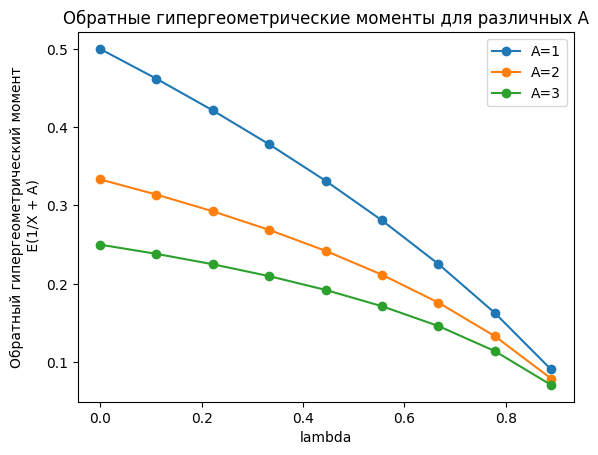
\includegraphics[width=12cm]{images/output1.png}
    \caption{ Обратный гипергеометрический момент при разные значения $\lambda$ }
    \label{hypergeo_fig}
\end{figure}

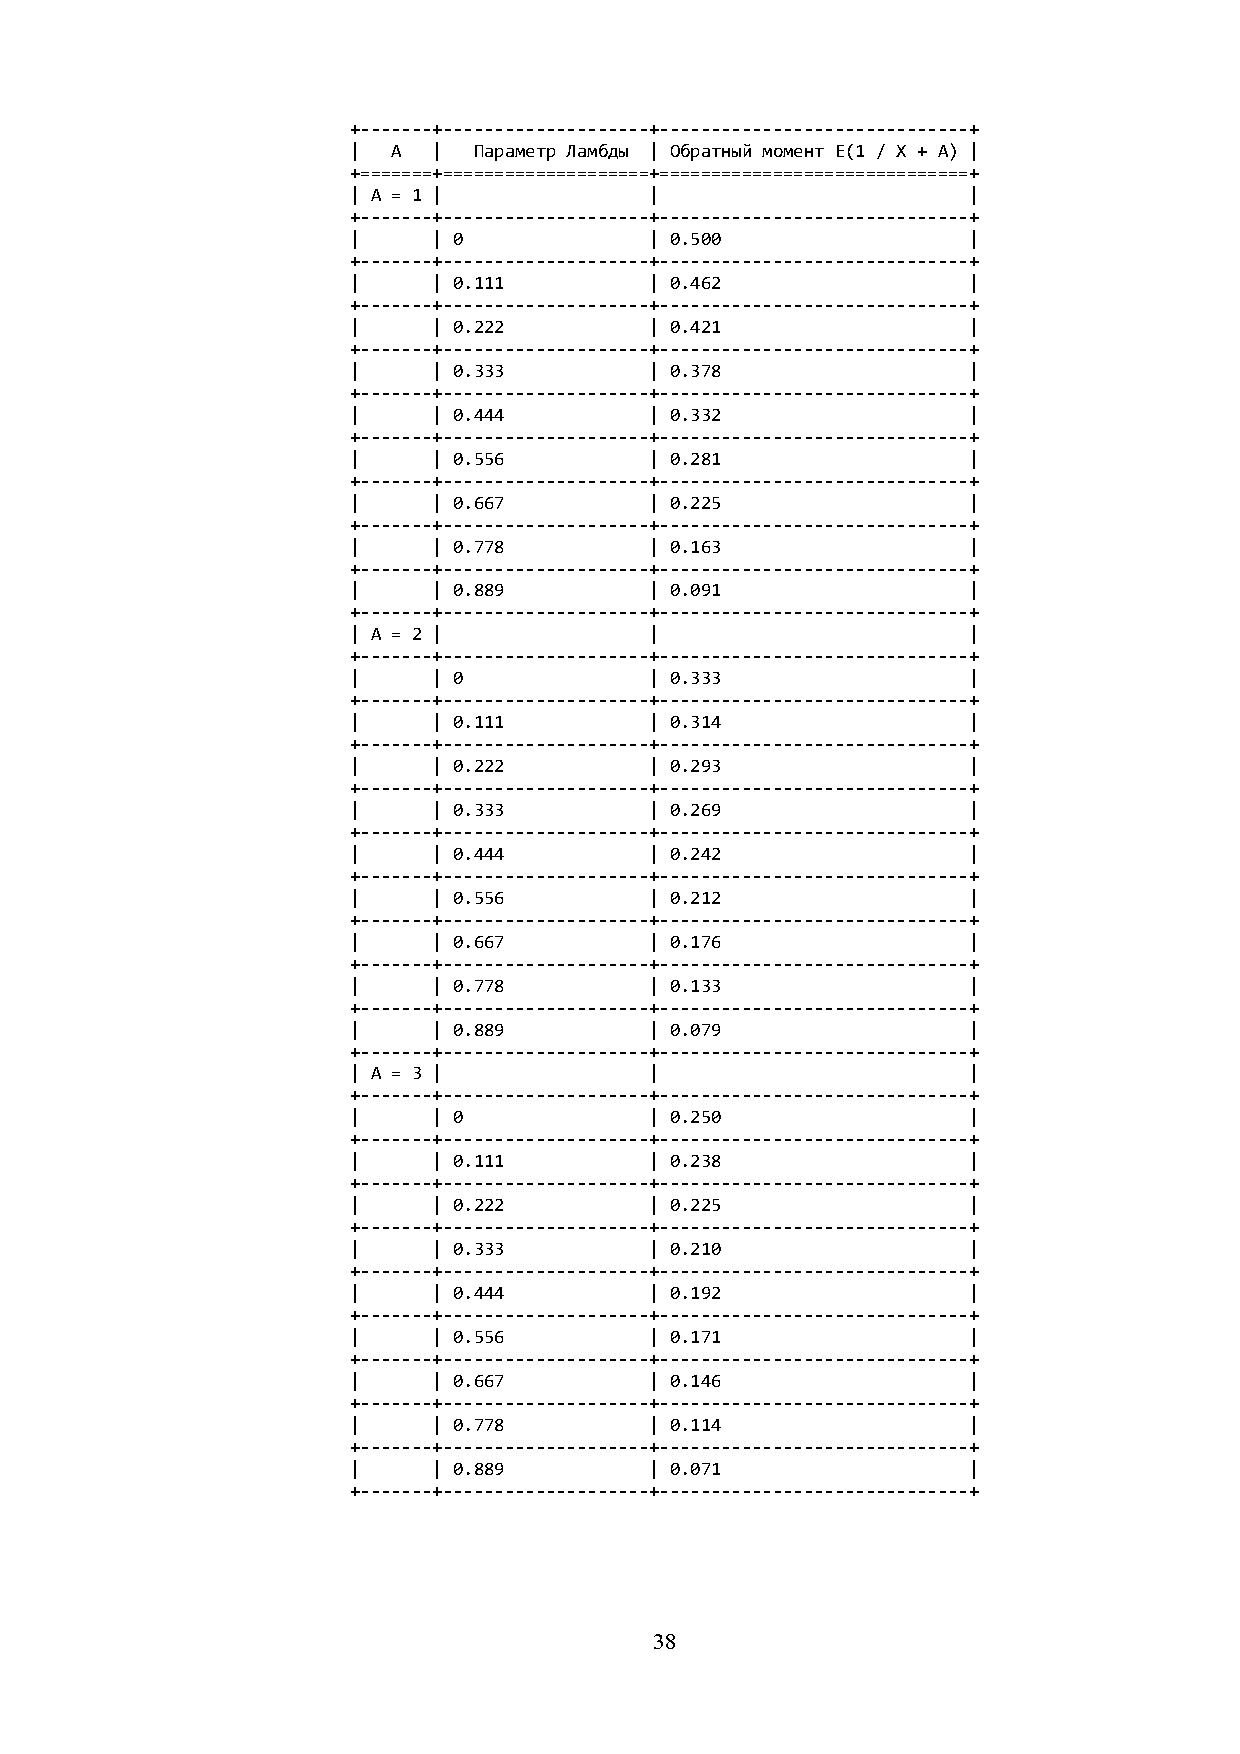
\includepdf[pages = 1]{data/result_hypergeome.pdf}

\newpage
\subsubsection{Методы расчета и использование биномаильних обратных моментов}

На основе исследований, проведенных в разделе (\ref{subsection 2.2}), касающемся получения обратных моментов через формулы (\ref{14}) случае когда случайная величина, определенная по вероятности в пространстве $(x,\alpha,P)$ имеет вид $E\big(\frac{1}{X}\big) \approx E\big(\frac{1}{A + X}\big)$ . Затем были получены  после вычисления различных значений выборок $n$ и с вероятностью успеха $p=0,5$. Который наглядно представлен первой таблицей и графиками, иллюстрирующими широкий спектр изменений обратного момента биномиального распределения $E\big(\frac{1}{X}\big)$. Вторая таблица дает изменение обратного момента биномиального распределения с теми же выборками и вероятностями успеха, но на этот раз в соответствии с целым числом $A$, которое принимает значения от $1$ до $3$.
\begin{equation*}
     E\bigg(\frac{1}{X+1}\bigg)=\frac{(1-(1-p)^{n+1})}{p(n+1)}=\frac{1-q^{n+1}}{p(n+1)}, 
\end{equation*}
где $p$ - вероятность успеха;\par
$q=1-p$ - вероятность неудачи или неуспеха и $n$ - выборки испытаний.
\vspace{6 mm}
\begin{figure}[htp]
    \centering
    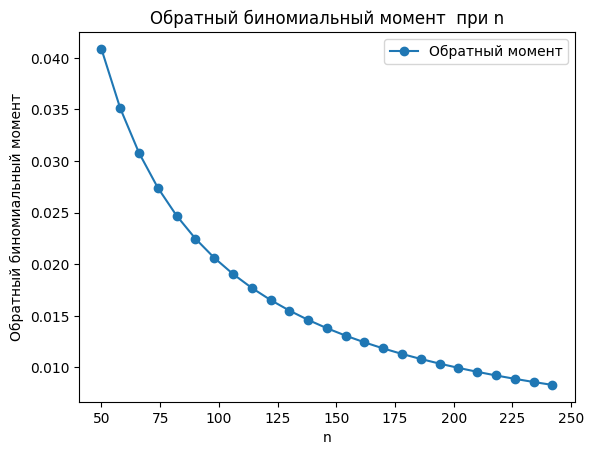
\includegraphics[width=12cm]{images/moment_inverse_bino.png}
    \caption{ Обратный биномиальный момент при разные значения $n$ }
    \label{binom_fig}
\end{figure}

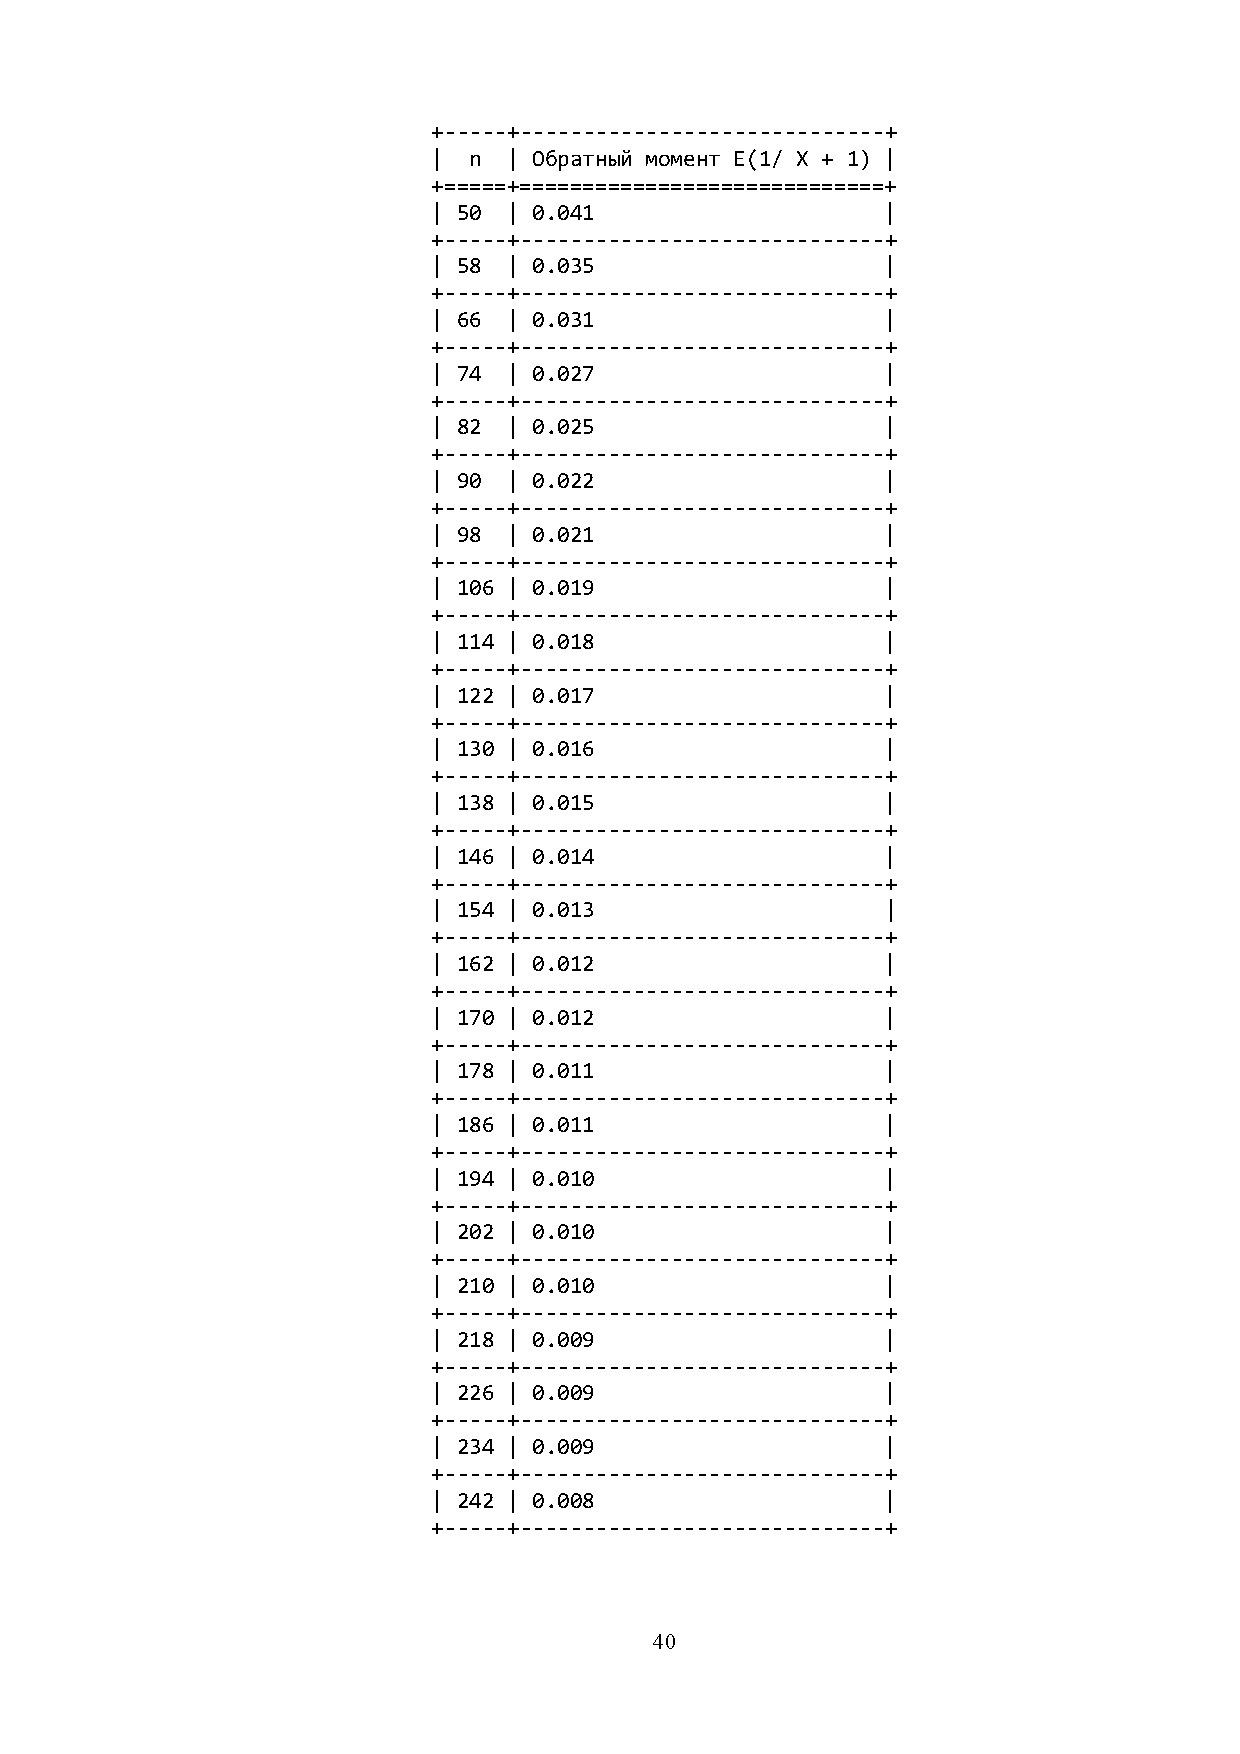
\includepdf[pages = 1]{data/bino.pdf}

\vspace{6 mm}
\begin{figure}[htp]
    \centering
    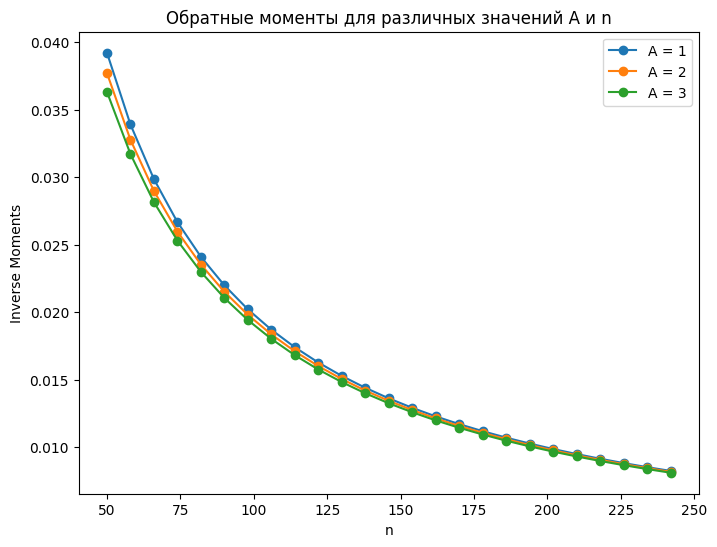
\includegraphics[width=12cm]{images/output3_inverse_binonial.png}
    \caption{ Обратный биномиальный момент при разные значения $n$ и $A$ }
    \label{binom_fig2}
\end{figure}

\vspace{3 mm}
\begin{figure}[htp]
    \centering
    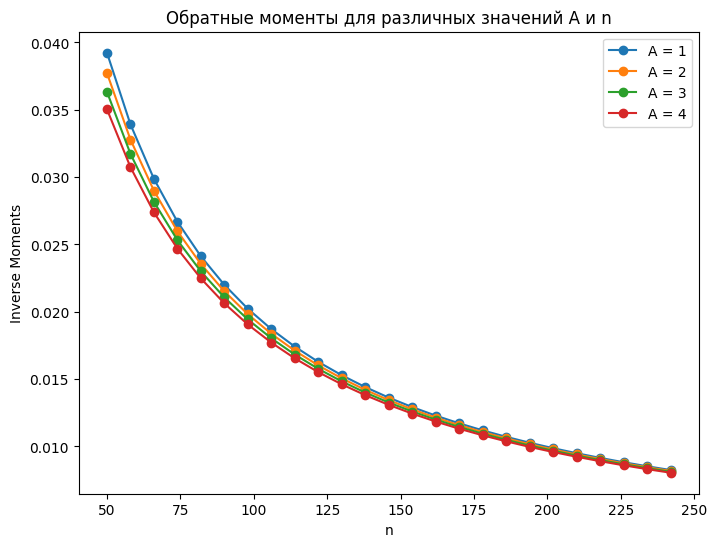
\includegraphics[width=10cm]{images/moment.png}
    \caption{ Обратный биномиальный момент при разные значения $n$ и $A$ }
    \label{binom_fig3}
\end{figure}

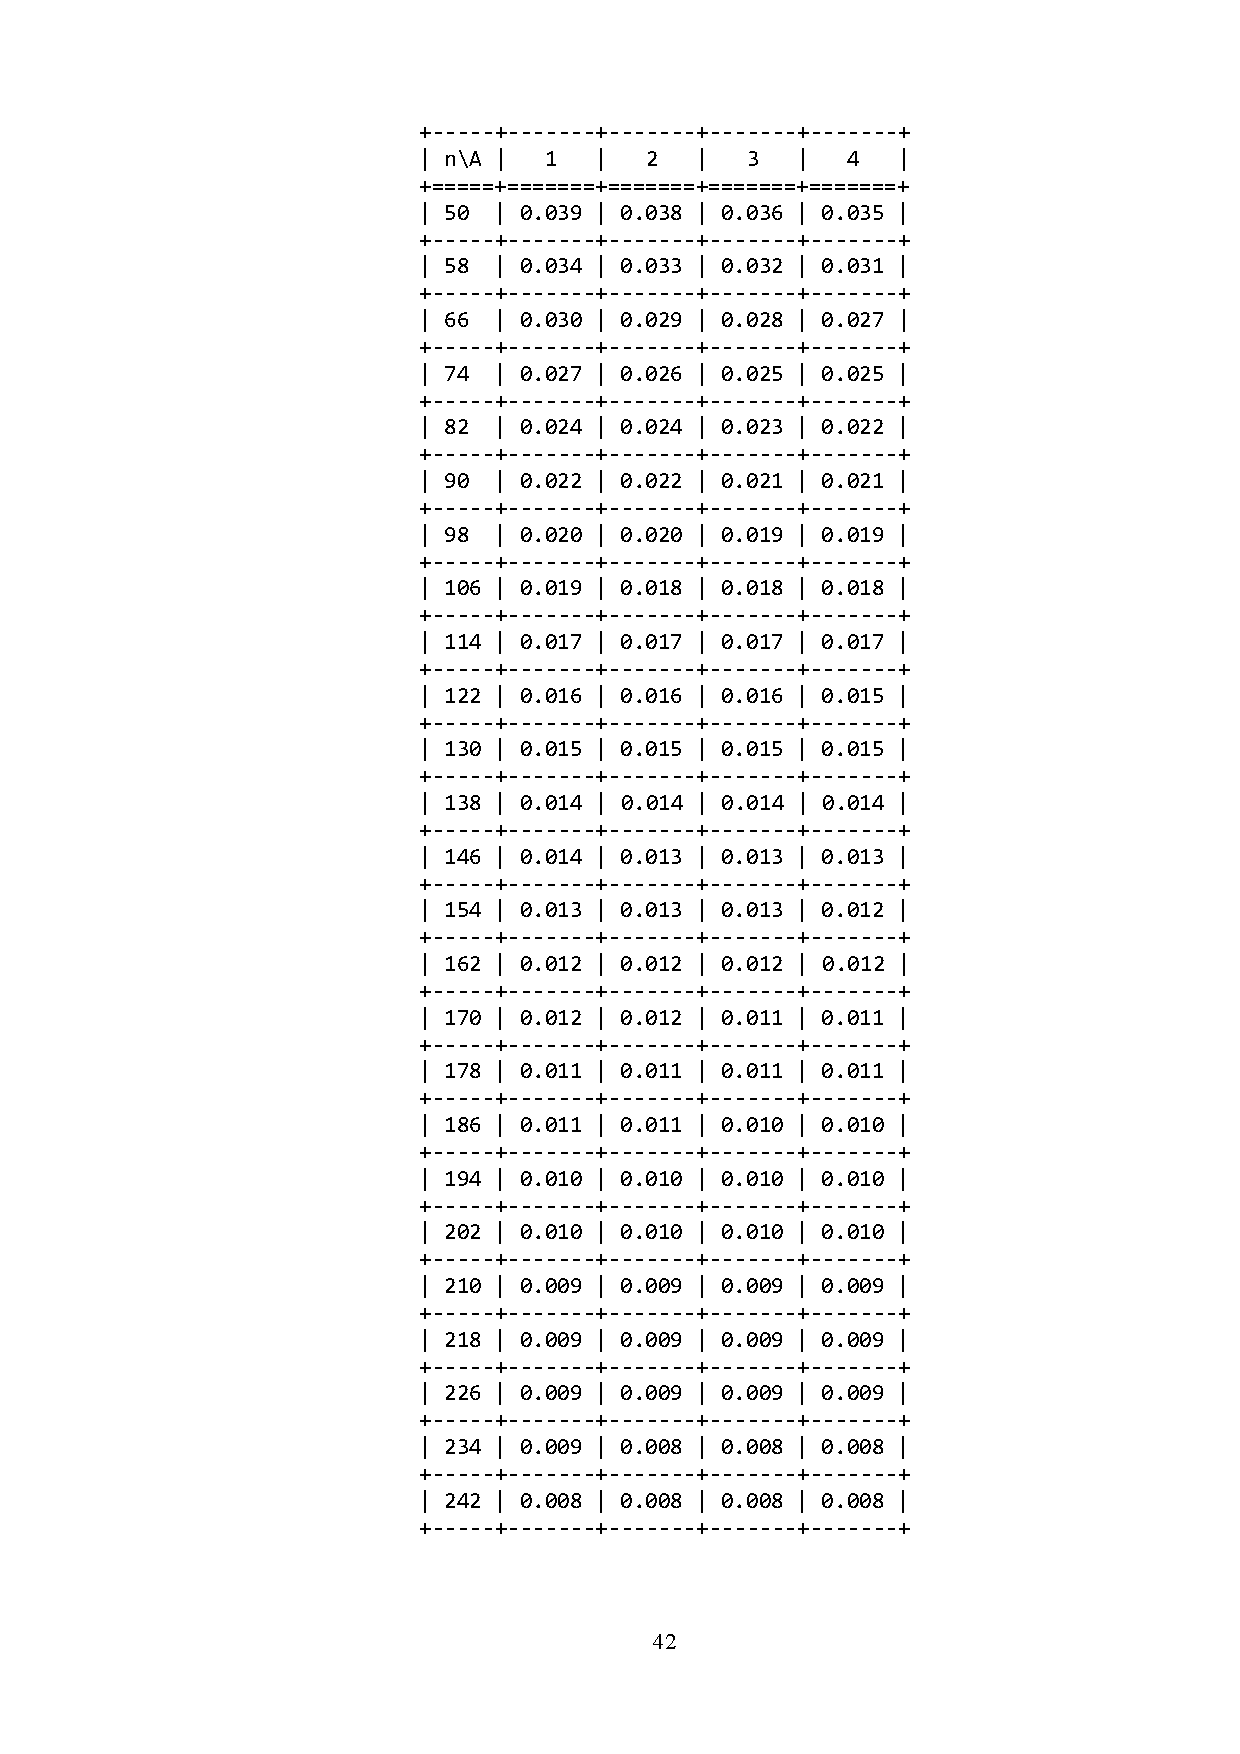
\includepdf[pages = 1]{data/X_inverse1.pdf}

\subsubsection{Методы расчета и использование обратных моментов Пуассона}
Как и другие дискретные распределения, распределение Пуассона также допускает некоторые сложности при определении обратного момента аналитически. Однако, вычислив с помощью формулы, полученные в разделах (\ref{subsection 2.3}), как (\ref{eq:(22)}), что позволяет нам определить обратный момент, когда случайная величина распределяется по распределению Пуассона с параметрами $\lambda$ и, следовательно, $E(\frac{1}{X})$. А также когда случайная величина определяется по вероятности в пространстве $(x, \alpha, p)$, то есть $E( \frac{1}{X+A})$ по следующей формуле (\ref{eq::25}), (\ref{eq::26}), (\ref{eq::27}), (\ref{eq::29}), с помощью которых осуществляется определение обратных моментов со значениями целых чисел А.
\begin{equation*}
    E\bigg(\frac{1}{X}\bigg) = e^{-\lambda} \sum_{n=1}^{\infty} \frac{\lambda^{n}}{n!} \frac{1}{n}
\end{equation*}

\begin{equation*}
E\Big(\frac{1}{X+1}\Big)=\frac{1-e^{-\lambda}}{\lambda}.
\end{equation*}

\begin{equation*}
    E\Big(\frac{1}{X+A}\Big) = \frac{1}{\lambda}\Bigg[1+\sum_{j=1}^{r}\frac{\prod_{i=1}^{j}(A-i)}{\lambda^{j}}(-1)^{J}+(-1)^{r+1}\frac{\prod_{i=1}^{j}(A-i)}{\lambda^{r}}E\Big(\frac{1}{X+A-r-1}\Big)\Bigg].
\end{equation*}
Была вычислена первая формула (\ref{eq:(22)}) для параметров $\lambda$, принимающая значения от $1, \cdots, 12$. и вторая таблица в соответствии с формулой (\ref{eq::25}), (\ref{eq::26}), (\ref{eq::27}), (\ref{eq::29}) , когда мы получаем разные значения.

\vspace{6 mm}
\begin{figure}[htp]
    \centering
    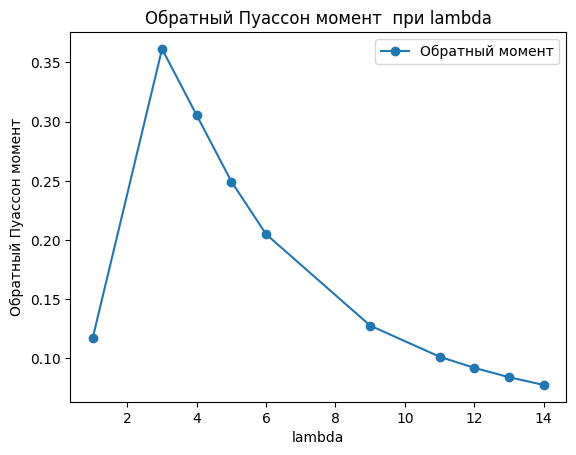
\includegraphics[width=12cm]{images/poisson.png}
    \caption{ Обратный Пуассон момент при разные значения $\lambda$ }
    \label{poisson_fig}
\end{figure}
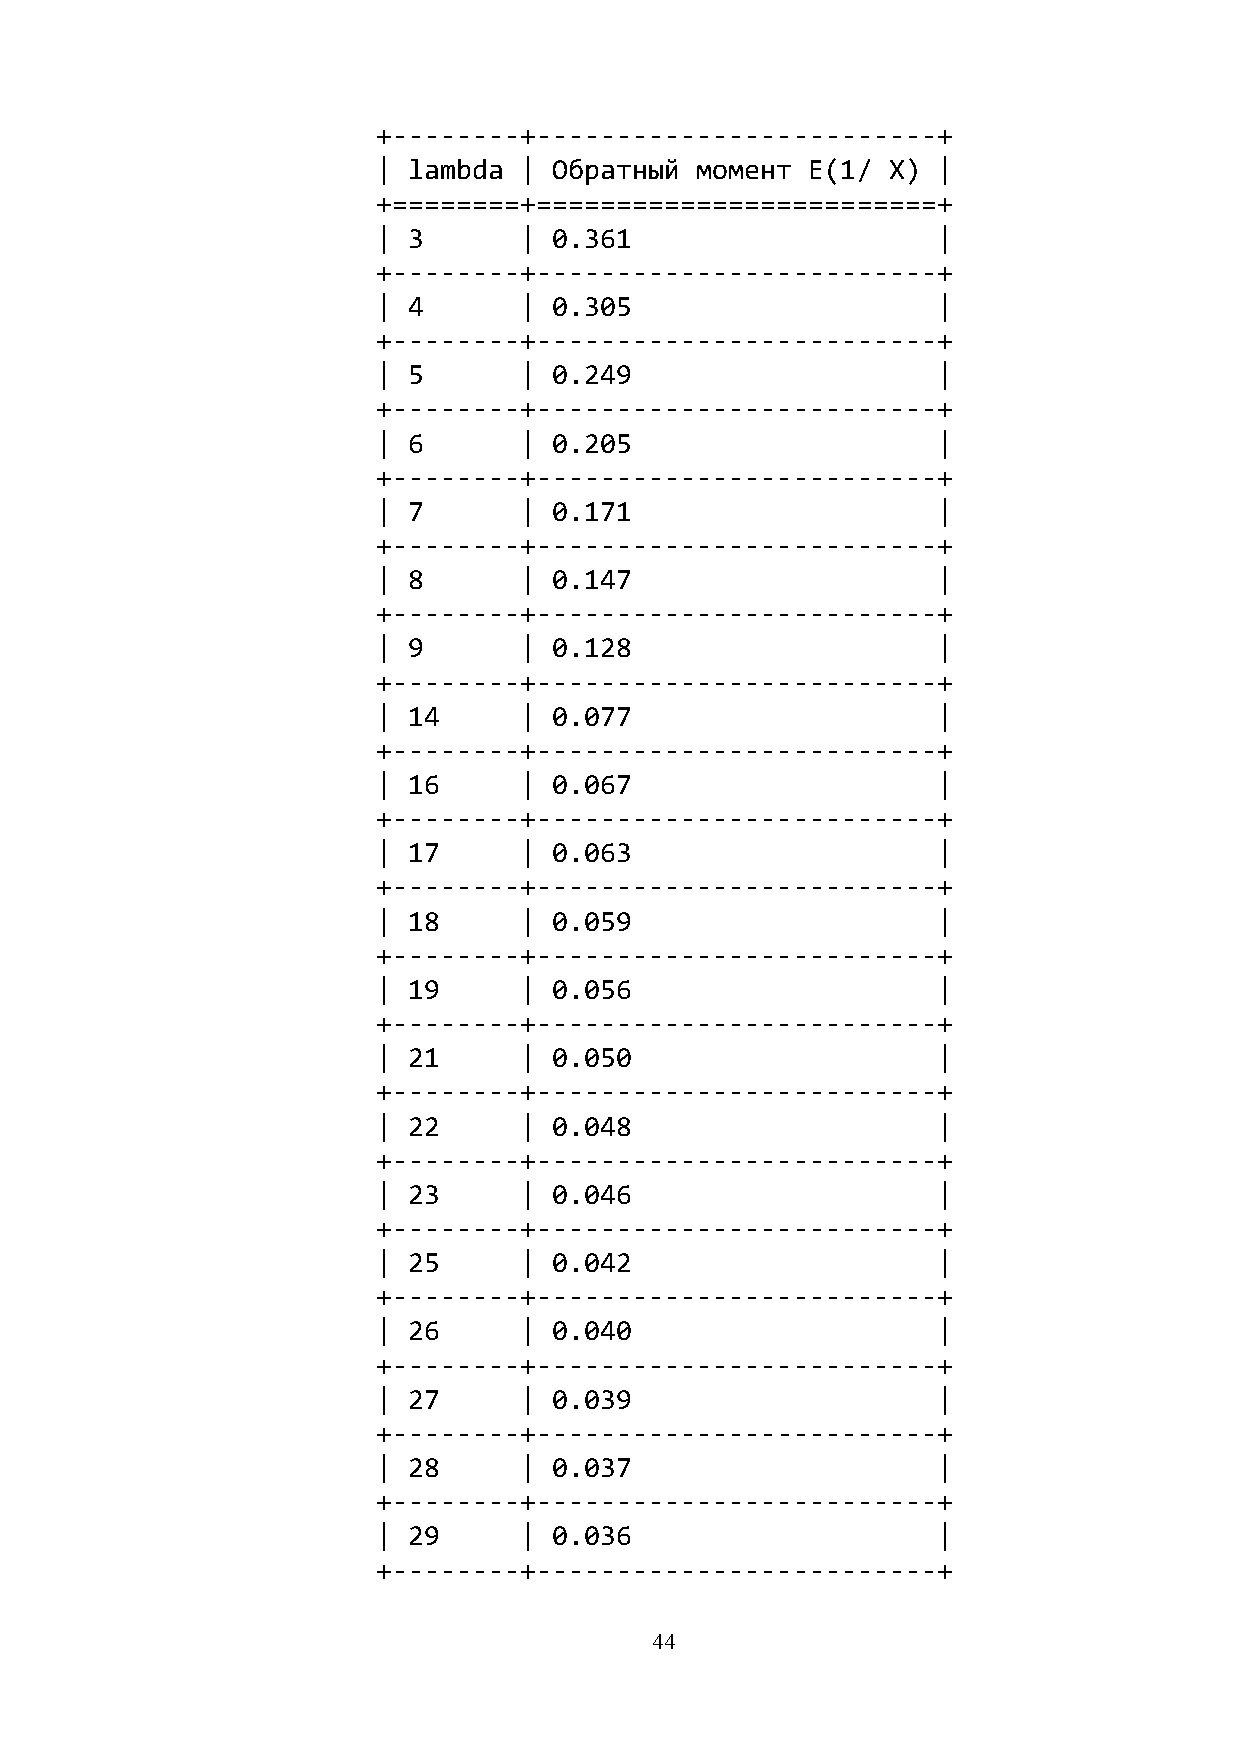
\includepdf[pages = 1]{data/X_inverse2.pdf}

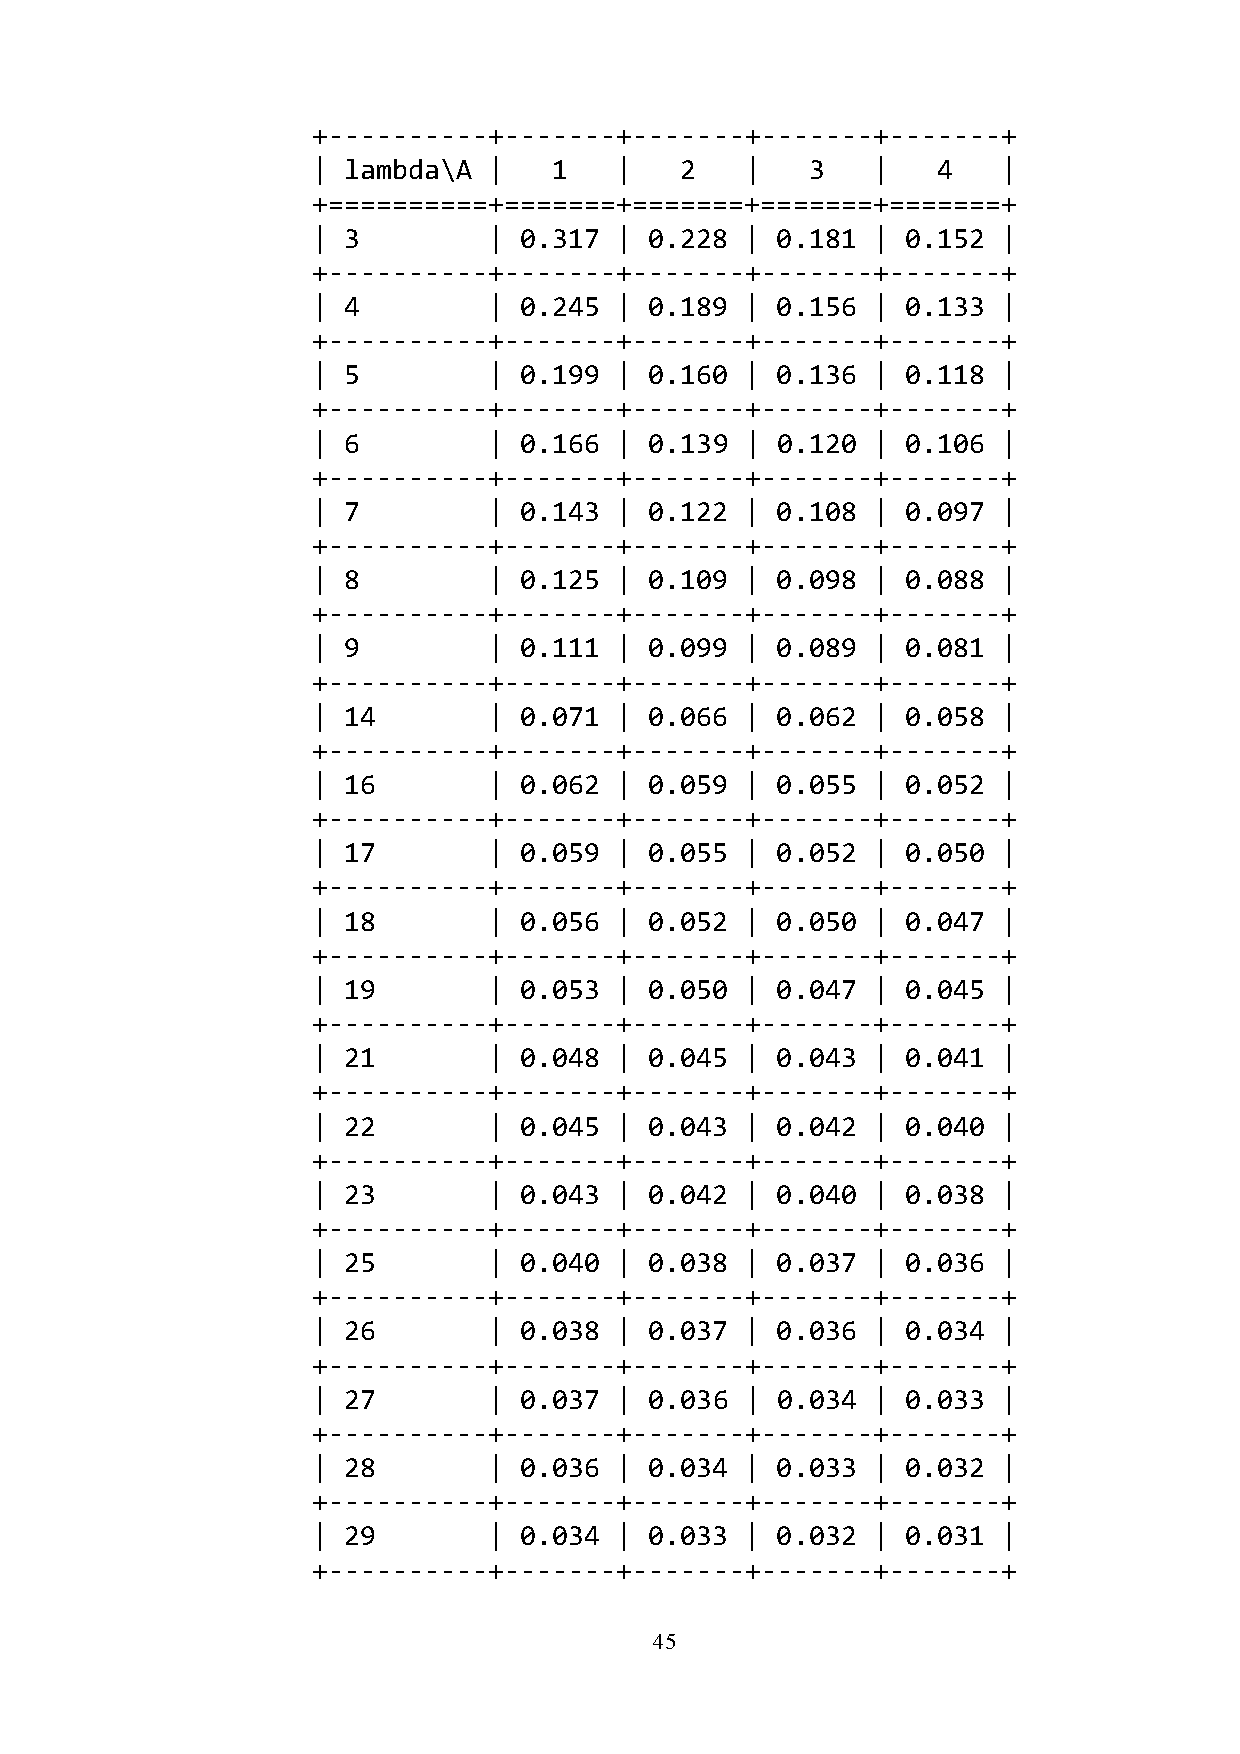
\includepdf[pages = 1]{data/X_inverse3.pdf}

\vspace{10 mm}
\begin{figure}[htp]
    \centering
    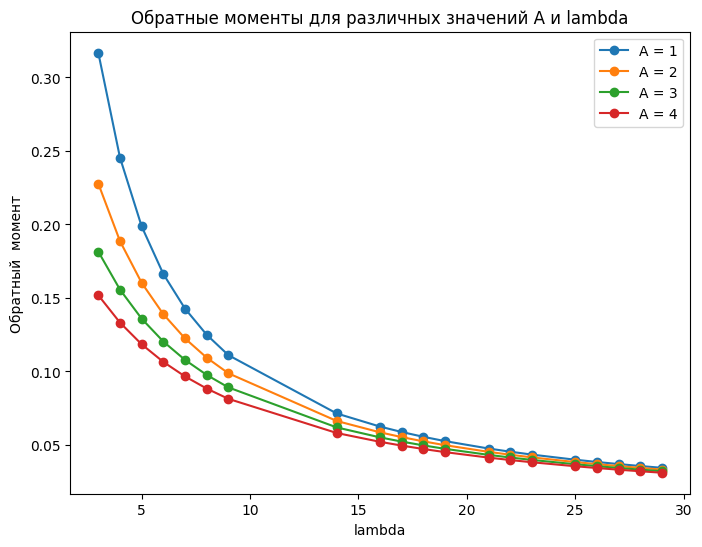
\includegraphics[width=14 cm]{images/poisson2.png}
    \caption{ Обратный Пуассон момент при разные значения $\lambda$ }
    \label{poisson_fig}
\end{figure}
\vspace{10 mm}

\subsubsection{Методы расчета и использование обратного моментов гамма-распределения }

Случайная величина X, распределенная в соответствии с вероятностью гамма-распределения, имеет обратный момент, когда $E(1/X)$ и может быть найдена по формуле (\ref{eq:30}).
\begin{equation*}
    E\bigg(\frac{1}{X}\bigg) =\frac{\beta}{\alpha - 1}.
\end{equation*}
Однако, когда случайная величина определяется по вероятности в пространстве $(x, \alpha, p)$, следовательно, обратный момент $E\big( \frac{1}{X+A}\big)$ можно определить с помощью формул (\ref{eq:31}) и (\ref{eq:32}), в зависимости от значения целого числа $A$ относительно, когда $A = 1$ и $ A > 1$. Формулы, которые получаются путем интеграции производящией функции моментов в разделе (\ref{subsection 2.4}).
\begin{equation*}
    E\bigg[\frac{1}{(X+A)^{r}}\bigg] = \frac{1}{\Gamma(r)} \int_{0}^{\infty}t^{r-1}e^{-At}M_{X}(-t)dt.
\end{equation*}
При $r=1$:
\begin{equation*}
    E\bigg[\frac{1}{X+A}\bigg] =  \int_{0}^{\infty}e^{-At}M_{X}(-t)dt 
\end{equation*}
Таким образом, в процедуре вычисления обратного момента гамма-распределения с параметрами: $\alpha$ - формы параметров, которые принимают свое значение случайным образом, а также $\beta$ - шкалы параметров, которые принимают значения $2,3,4$ . таким образом, мы можем заметить на каждом графике изменения в зависимости от параметра $\alpha$, изменения в моментах в обратном порядке, а также перевод в табуляцию, и второй график, который иллюстрирует определение, когда мы $E(1 / X+ A)$.

\vspace{10 mm}
\begin{figure}[htp]
    \centering
    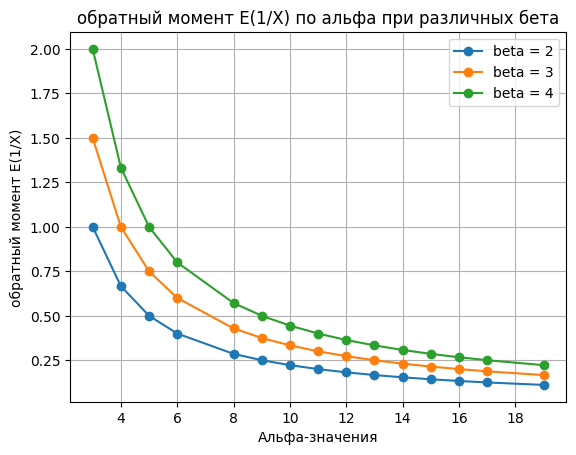
\includegraphics[width=14 cm]{images/gamma1.png}
    \caption{ Обратный момент Гамма-распределения при разные значения $\lambda$ и $\beta$ }
    \label{gamma_fig}
\end{figure}
\vspace{10 mm}
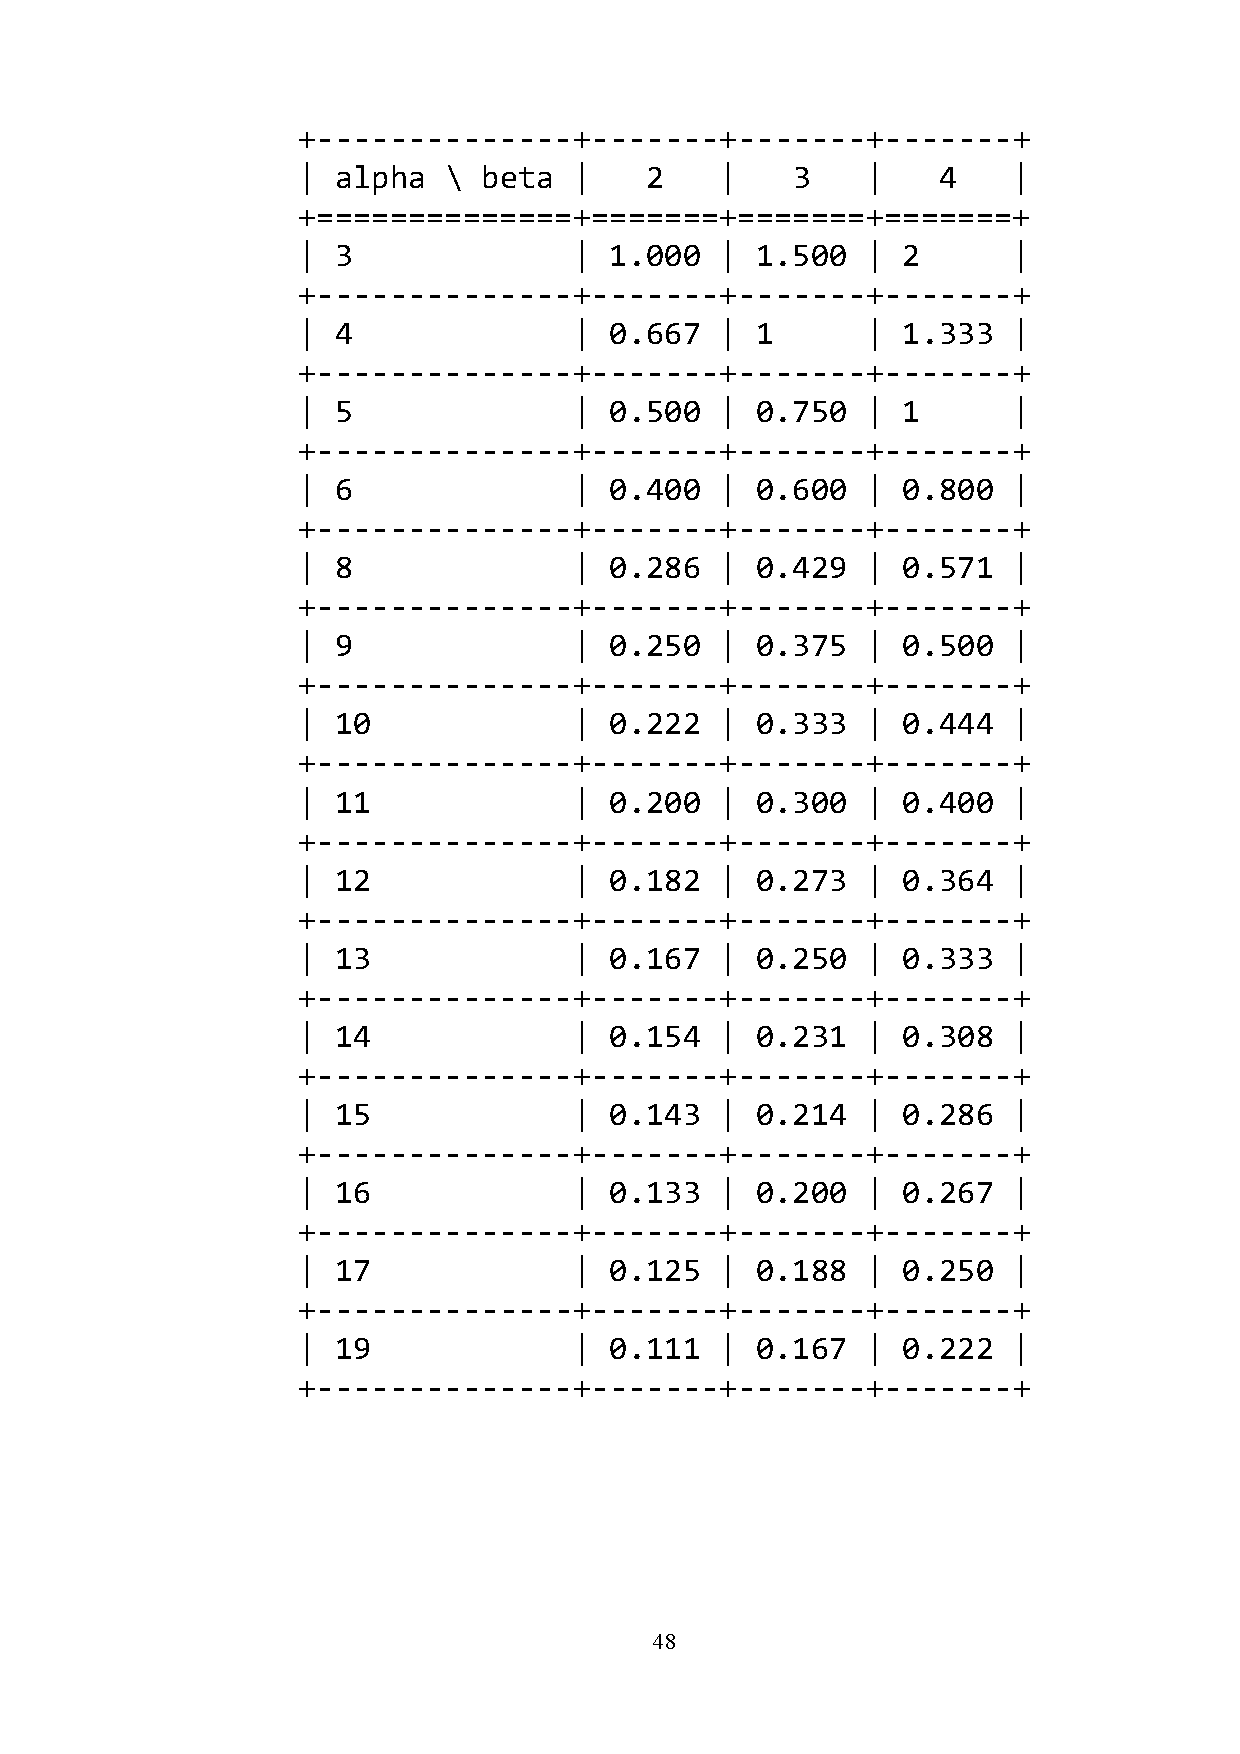
\includepdf[pages = 1]{data/gamm1.pdf}

\vspace{10 mm}
\begin{figure}[htp]
    \centering
    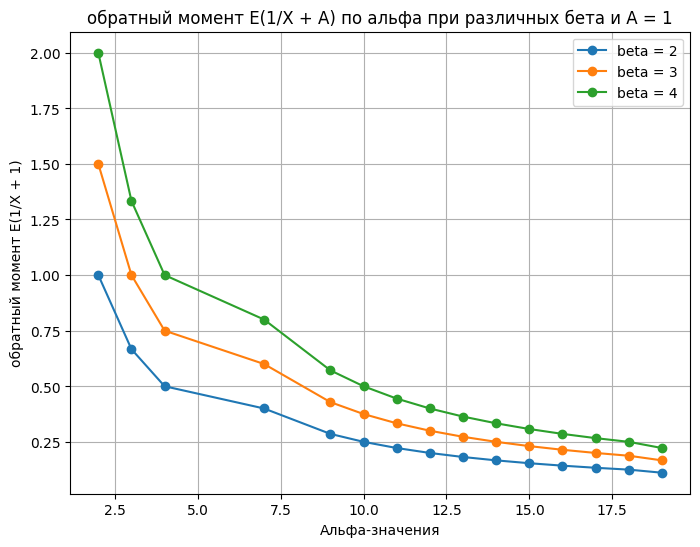
\includegraphics[width=11 cm]{images/gamma2.png}
    \caption{ Обратный момент Гамма-распределения при разные значения $\lambda$ и $\beta$ }
    \label{gamma_fig2}
\end{figure}
\vspace{10 mm}

\begin{figure}[htp]
    \centering
    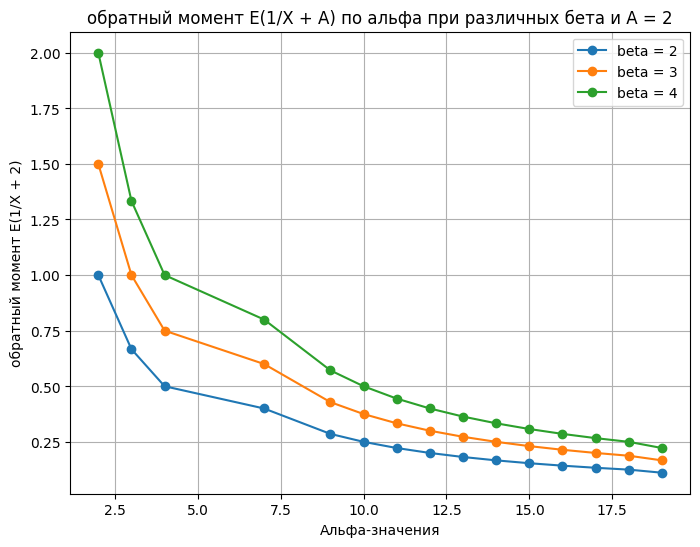
\includegraphics[width=11.5 cm]{images/gamma3.png}
    \caption{ Обратный момент Гамма-распределения при разные значения $\lambda$ и $\beta$ }
    \label{gamma_fig3}
\end{figure}

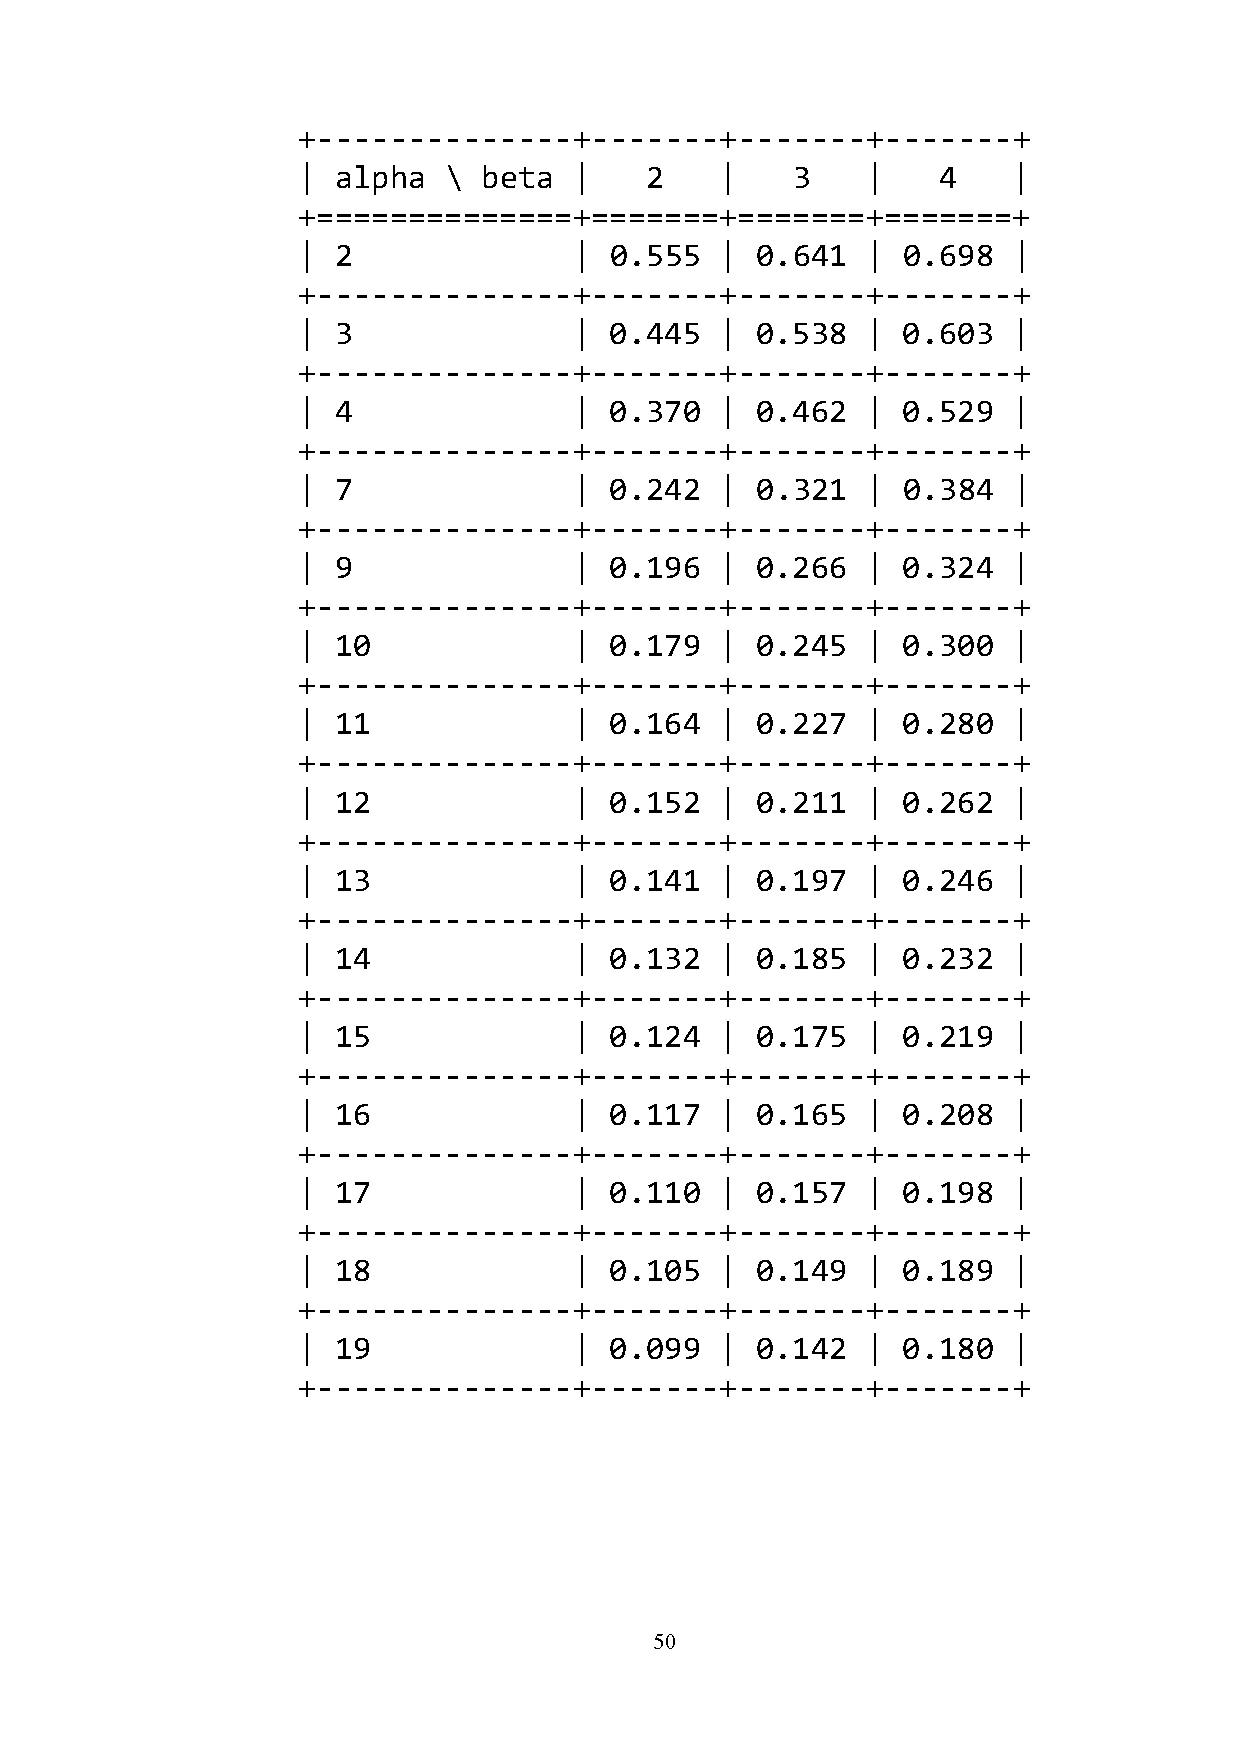
\includepdf[pages = 1]{data/gamm2.pdf}

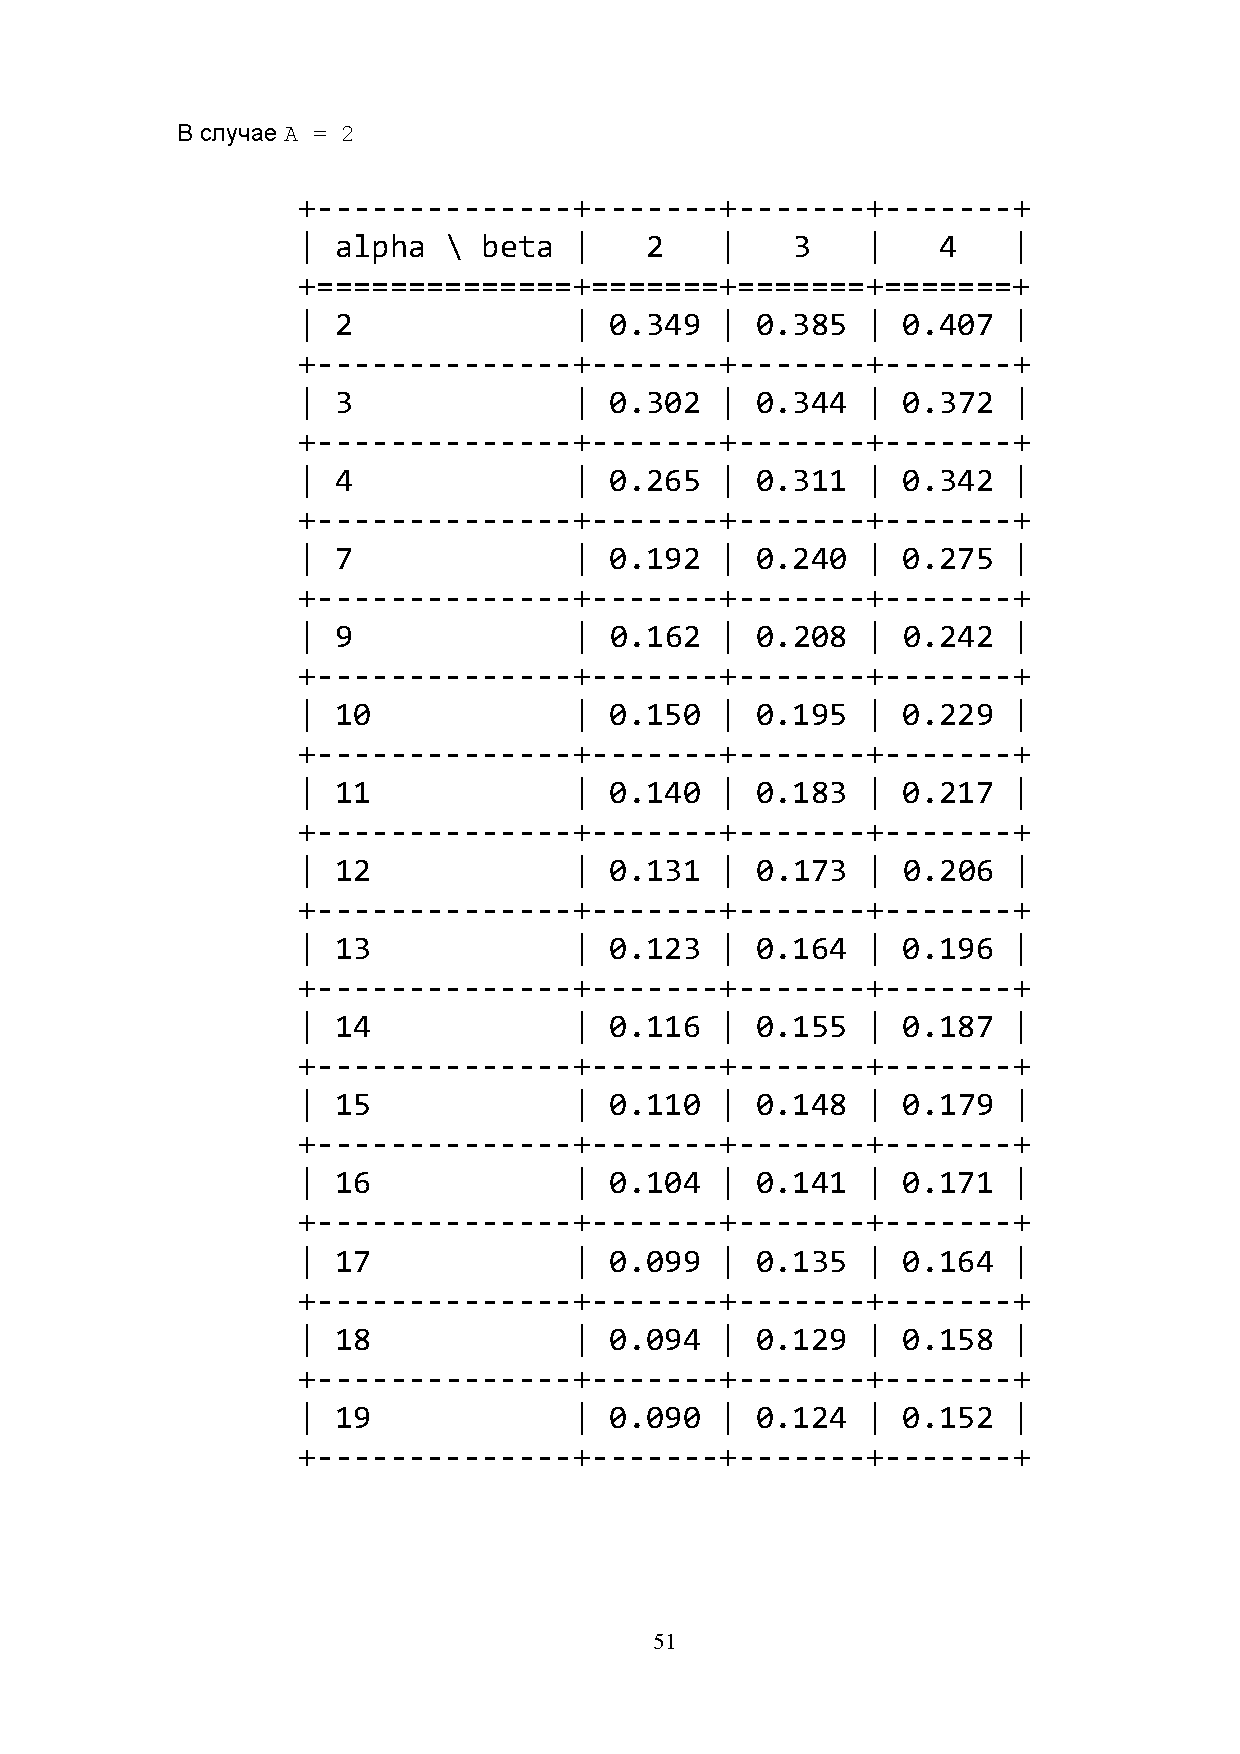
\includepdf[pages = 1]{data/gamm3.pdf}


\newpage
\section{Заключение}\label{section 4}
В ходе данной работы был дан литературный обзор, обратного момента случайных величин статистических распределений и, в частности, гипергеометрического, биномиального, пуассоновского, экспоненциального, гамма- и бета-распределений. Таким образом, обратный момент случайной величины в распределении-это переменная, которую мы также можем получить, интегрировав от 0 до бесконечности производящую функцию момента этого же распределения. Во всех случаях, в зависимости от характера статистического распределения, момент может быть неопределимым, как хорошо заметили в случае экспоненциального распределения. Oно также может быть определен под порядком, то есть обратный момент первого порядка, второго порядка и так далее. Однако определить обратный момент второго порядка, перейдя в порядок $r$, не всегда легко, поскольку некоторые распределения не имеют бесконечно конечных значений.


В целом Обратный момент случайных величин статистических распределений относится к статистической мере, включающей обратные значения случайной величины, возведенные в заданную степень. Он специально определен для случайной величины $X$ как $E(X ^{-r})$, где $r$-ого, положительное целое число, представляющее степень математическое ожидание $X$. Проще говоря, он измеряет ожидаемое значение обратной величины переменной, возведенной в степень. Следуя этого первой обратной момент принимает вид при $r=1$, то есть $E[X^{-1}]$. Обратной момент часто используется в таких областях, как экономика, финансы и страхование, где понимание поведения обратных величин случайных величин может быть особенно важным. Важно отметить, что обратные моменты существуют только в том случае, если ожидаемые значения конечны, для чего обычно требуется случайная величина $X$ быть строго позитивным ($X > 0$ ), чтобы избежать деления на ноль или неопределенного поведения. Как и другие переменные( математическое ожиданое), обратный момент случайной величины также имеется нескольких свойства: линейность, сложность и условность. 

В среде языка программирования python было выполнено вычисление метода определения обратного момента случайной величины, поскольку не всегда очень очевидно получить более точный и описательный результат соответствующего распределения аналитически. было замечено, что после аналитического и вычислительного определения некоторые распределения имеют обратный момент, такой как распределение Пуассона, биномиальное распределение, гамма-распределение и бета-распределение. С другой стороны, другие, такие как экспоненциальное распределение, не имеют обратного момента. Таким образом, обратный момент является функцией, уменьшающей вероятность его распределения от случайной величины, т. е. чем больше возрастает значение параметра распределения, тем больше уменьшается значение обратного момента. Четко можно отметить  на различных графиках, полученных при вычислении обратного момента. На графике (\ref{hypergeo_fig}) который дает представление обратного момента случайной величины гипергеометрического распределения, показано иллюстрацию убывающие кривые в зависимости от возрастающего значения параметра лямбда, Этот же недостаток заметен и в других распределений на графике (\ref{binom_fig}), (\ref{gamma_fig}). 

Таким образом, в рамках данной работы :\par 
\begin{itemize}
    \item  Наблюдение и теоретическое изучение обратного момента случайной величины во всех ее формах, а также описание метода получения на основе каждого статистического распределения, определяющего эту случайную величину. Подчеркивание важности обратного момента в нескольких сферах деятельности, а также области его применения.\par
    \item Подстановка задач и изучение анитичесий и вычислительный метод расчёта обратных моментов разных распределний. 
    \item Представление результатов получены при использовании программной реализации.
\end{itemize} 

\newpage

\printbibliography

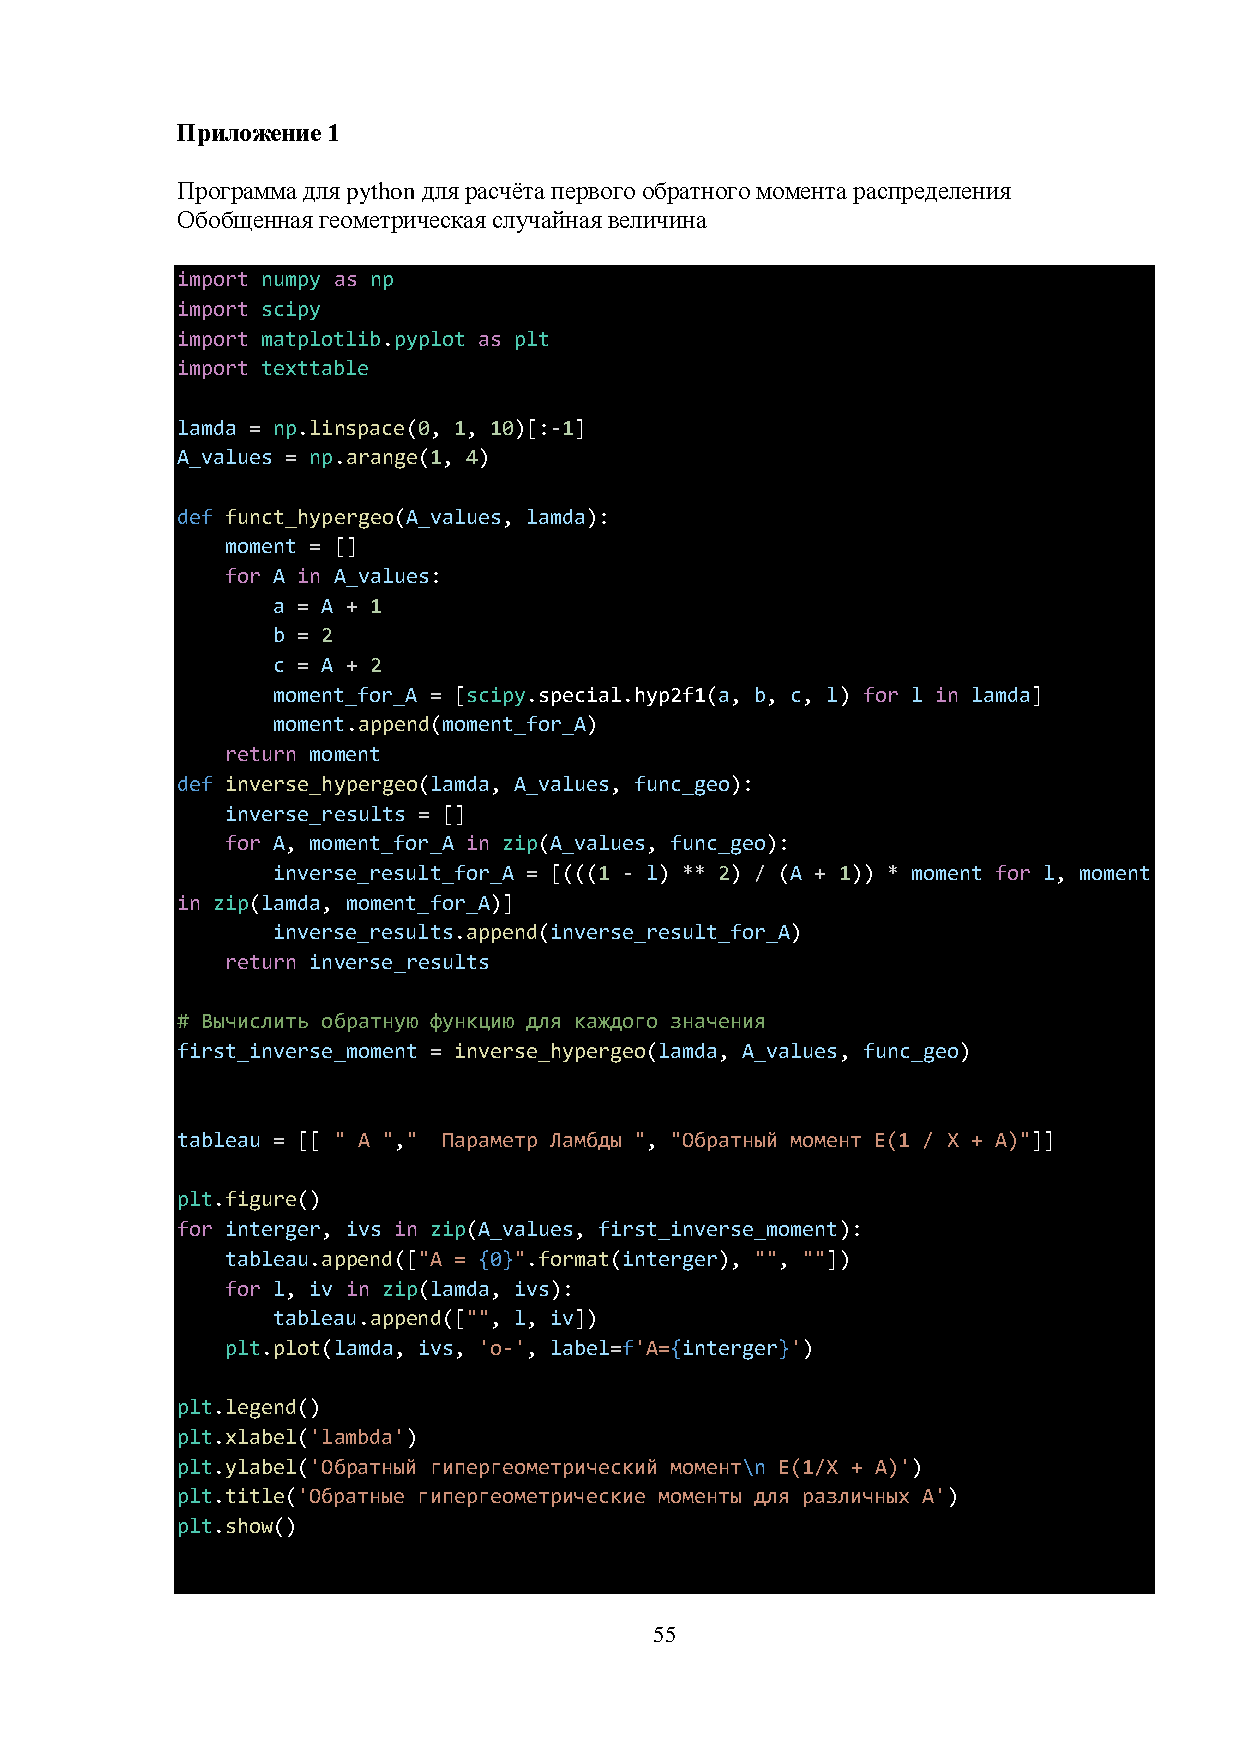
\includepdf[pages = 1-9]{data/Приложение.pdf}

\end{document}